\documentclass[11pt]{article}
\usepackage{geometry}                
\geometry{letterpaper}                   

\usepackage{natbib}

%\usepackage[latin1]{inputenc}
%\usepackage[english]{babel}
%\usepackage[T1]{fontenc} 

\usepackage{multirow}
\usepackage{lscape} % stellenweises Querformat TABLE

\usepackage{graphicx}
\usepackage{amssymb}
\usepackage{epstopdf}
\usepackage{natbib}
\usepackage{amssymb, amsmath}
\DeclareGraphicsRule{.tif}{png}{.png}{`convert #1 `dirname #1`/`basename #1 .tif`.png}

%\title{Title}
%\author{Name 1, Name 2}
%\date{date} 

\begin{document}



\thispagestyle{empty}

\begin{center}

\includegraphics[width=5cm]{ETHlogo.eps}

\bigskip


\bigskip


\bigskip


\LARGE{ 	Lecture with Computer Exercises:\\ }
\LARGE{ Modelling and Simulating Social Systems with MATLAB\\}

\bigskip

\bigskip

\small{Project Report}\\

\bigskip

\bigskip

\bigskip

\bigskip


\begin{tabular}{|c|}
\hline
\\
\textbf{\LARGE{Insert Title Here}}\\
\textbf{\LARGE{...}}\\
\\
\hline
\end{tabular}
\bigskip

\bigskip

\bigskip

\LARGE{Name 1 \& Name 2}



\bigskip

\bigskip

\bigskip

\bigskip

\bigskip

\bigskip

\bigskip

\bigskip

Zurich\\
May 2008\\

\end{center}



\newpage

%%%%%%%%%%%%%%%%%%%%%%%%%%%%%%%%%%%%%%%%%%%%%%%%%

\newpage
\section*{Agreement for free-download}
\bigskip


\bigskip


\large We hereby agree to make our source code for this project freely available for download from the web pages of the SOMS chair. Furthermore, we assure that all source code is written by ourselves and is not violating any copyright restrictions. We clearly state in the text, which external packages we used that were not written by ourselves. Those packages are freely available at Matlab FileExchange and are published under a BSU license. 
\begin{center}

\bigskip


\bigskip


\begin{tabular}{@{}p{3.3cm}@{}p{6cm}@{}@{}p{6cm}@{}}
\begin{minipage}{3cm}

\end{minipage}
&
\begin{minipage}{6cm}
\vspace{2mm} \large Fabio Crameri

 %\vspace{\baselineskip}

\end{minipage}
&
\begin{minipage}{6cm}

\vspace{2mm} \large Marcel Thielmann

\end{minipage}
\end{tabular}


\end{center}
\newpage

%%%%%%%%%%%%%%%%%%%%%%%%%%%%%%%%%%%%%%%



% IMPORTANT
% you MUST include the ETH declaration of originality here; it is available for download on the course website or at http://www.ethz.ch/faculty/exams/plagiarism/index_EN; it can be printed as pdf and should be filled out in handwriting


%%%%%%%%%% Table of content %%%%%%%%%%%%%%%%%

\tableofcontents

\newpage

%%%%%%%%%%%%%%%%%%%%%%%%%%%%%%%%%%%%%%%



\section{Abstract}



\section{Individual contributions}
No one wrote the individual contributions.

\section{Introduction and Motivations}

\section{Description of the Model}

\subsection{Agent}

The agents in our model represent ordinary pedestrians that are panically trying to derive an exit. Number, size, mass and max. velocity of each agent can be changed for different model setups. The agents are subject to different forces that are social and physical forces from other agents and from surrounding walls.

\subsubsection{Psychological forces}

Except for special circumstances, people do not like to move too close to each other. This can be represented by a repulsive force of a pedestrian to another. The psychologic social forces between two agents that are not touching each other can thus be described as

\begin{equation}
	{{\bf f}_{ijS}} = \left\{ {{A_i}\exp \left[ {\frac{{\left( {{r_{ij}} - {d_{ij}}} \right)}}{{{B_i}}}} \right] } \right\}{{\bf n}_{ij}} 
		\label{eq:fijS}
\end{equation}

where $A_i$ and $B_i$ are constants, ${\bf n}_{ij} = ({\bf r}_i - {\bf r}_j)/d_{ij}$ is the normalized vector pointing from pedestrian $j$ to pedestrian $i$, $d_{ij}$ is the distance between the pedestrians center of mass and $r_i$ is the size (i.e. radius) of the pedestrian \citep{Helbing2000}. 

\subsubsection{Physical forces}

In the case of physical contact between two pedestrians, there is two forces which one has to consider for a model of the present study. There is the normal force acting between the two colliding bodies, preventing them to merge, which can be formulated as

\begin{equation}
	{{\bf f}_{ijPn}} = {kg\left( {{r_{ij}} - {d_{ij}}} \right)} {{\bf n}_{ij}}
		\label{eq:fijPn}
\end{equation}

and a tangential force between two sliding agents given by

\begin{equation}
	{{\bf f}_{ijPt}} = \kappa g\left( {{r_{ij}} - {d_{ij}}} \right)\Delta v_{ji}^t{{\bf t}_{ij}} .
		\label{eq:fijPt}
\end{equation}

Here, the function $g$ is zero if the pedestrians do not touch each other, $k$ and $\kappa$ are large constants and $\Delta v_{ji}^t = ({\bf v}_j - {\bf v}_i)\cdot {\bf t}_{ij}$ is the tangential velocity difference \citep{Helbing2000}.

When the different forces are added together, we obtain the total social force applied on an agent

\begin{equation}
	{{\bf f}_{ij}} = {{\bf f}_{ijS}} + {{\bf f}_{ijPn}} + {{\bf f}_{ijPt}} .
		\label{eq:fij}
\end{equation}

\subsection{Walls}

For a pedestrian panic to occur, walls are needed. They bound a certain amount of space, which might become small when filled with people. They further produce bottlenecks at positions where a room suddenly gets smaller or where there is an exit at which pedestrians are accumulated. From nature we know two main behaviors regarding walls: People usually don't like to walk too close to a wall and people can not walk through a wall. Therefore there are two forces to consider, when modeling such a feature, psychologic and physical forces, respectively.

\subsubsection{Psychological forces}

The psychological repulsive force defined here for the walls/buildings can be written in mathematical terms as

\begin{equation}
	{{\bf f}_{iWS}} = \left\{ {{A_i}\exp \left[ {\frac{{\left( {{r_i} - {d_{iW}}} \right)}}{{{B_i}}}} \right]} \right\}{{\bf n}_{iW}} ,
	\label{eq:fiWS}
\end{equation}

where $A_i$ and $B_i$ are constants, $n_{iW}$ is the normalized vector pointing from the pedestrian to the wall, $d_{iW}$ is the distance in between and $r_i$ is the size (i.e. radius) of the pedestrian (Helbing et al., 2000).

\subsubsection{Physical forces}
As in the case of physical inter-agent forces, an agent is subject to physical forces from the walls if it comes too close to a wall. The physical wall forces can be divided into a normal force $f_{iWPn}$ and a tangential force $f_{iWPt}$ acting from the wall and are written as:

\begin{equation}
	{{\bf f}_{iWPn}} = \left\{ {kg\left( {{r_i} - {d_{iW}}} \right)} \right\}{{\bf n}_{iW}}
	\label{eq:fiWPn}
\end{equation}

and

\begin{equation}
	{{\bf f}_{iWPt}} = \left\{ {\kappa g\left( {{r_i} - {d_{iW}}} \right)\left( {{{\bf v}_i} \cdot {{\bf t}_{iW}}} \right)} \right\}{{\bf t}_{iW}} ,
	\label{eq:fiWPt}
\end{equation}

respectively. Here, the function $g$ is zero if the pedestrian does not touch the wall, $k$ and $\kappa$ are large constants and $(v_i \cdot t_{iW})$ is the tangential velocity difference.

The total repulsive force from the architecture $f_{iW}$ can then be written as

\begin{equation}
	{{\bf f}_{iW}} = {{\bf f}_{iWS}} + {{\bf f}_{iWPn}} - {{\bf f}_{iWPt}} .
	\label{eq:fiW}
\end{equation}



\subsection{Exits}
\label{sec:Exits1}

In our model, the sole attractive force is the exit force. As for the social forces, it is rather a psychological force representing the will of each agent to reach the exit. In this work, we chose the value of the exit force to be proportional to the sum of the other psychological forces (in our code, one can choose a proportionality constant to adjust the exit force). To determine the direction of the exit force, we used two different approaches: i) the agent is drawn directly towards the exit, regardless of any obstacles in between him and an exit, and ii) the agent decides on its walking direction based on the estimate of the time it needs to reach the exit (e.g. \citet{Graf,Kneidl}).

While i) is relatively straightforward to implement, there are several crucial drawbacks to this method: First, it does not reflect at all the decision process of a human agent, since obstacles between the agent and the exit are always taken into account. Second, 

\subsubsection{Shortest path formulation}

Finding the shortest path between two points is a mathematical problem that has received much attention since it's solution can be used in a huge number of applications. One of the earliest solutions to this problem was presented by Dykstra (reference). Shebian (right name? reference?) presented a fast and efficient method to solve a certain class of shortest path problems, which  is called the Fast marching method. It is a special case of level set methods and solve the Eikonal equation (equation?). In geophysics, the Eikonal equation is used to describe the 

This equation describes the We can essentially apply this algorithm to our problem

In a more sophisticated version of the code, we make use of a fast marching algorithm that takes into account walls as being regions with a low velocity. We compute the shortest path


\subsection{Flood}

In model cases were we use a rising flood, another repulsive force is added. The flood will rise with time and adjust laterally depending on the local topography. Agents will try to prevent going into water, but are able to walk through it until a certain depth level.

\subsection{Pedestrian walking speed}

The free (unobstructed by obstacles) walking speed of pedestrians is determined by several factors:

\begin{enumerate}
\item the conditions of the ground
\item the situation of an agent (e.g. panic)
\item the forces acting on an agent
\end{enumerate}

In our model, we assume the conditions of the ground to be the same everywhere, meaning that there is no effect of ground roughness on the velocity of the agent. However, as we intend to include topography in our model, we introduce a walking speed function that is dependent on the slope $S$ of the ground (TOBLER):

\begin{equation}
	v(S) = A_{S} \exp{\left( -B_S | S + S_{crit} |  \right)}\mbox{,}
\end{equation}

where $A_S$ and $B_{S}$ represent constant factors and $S_{crit}$ is the critical slope above which a pedestrian actually slows down while walking downwards (see also fig.\ref{fig:walking_speed}). TOBLER used values of $A_S = 6$, $B_S = 3.5$ and $S_{crit} = 0.05$. On flat terrain, those parameters result in a walking speed of 5 km/h., if $A_S$ is given in units of km/h. In panic situations however, this velocity can reach values of 5-6 m/s. Here, we take this into account by varying the factor $A_S$ in the walking speed function to account for higher velocities.

To account for the impact of psychological and physical forces on pedestrian walking speed, \citet{Helbing2000} used the following equation for the change of agent velocity in time:

\begin{equation}
	\frac{d \mathbf{v}_i}{dt} = \frac{v_i^0\mathbf{e}_i - v_i(t)}{\tau_i} - \sum_{j(\ne i)}f_{iW} - \sum_{j(\ne i)}f_{iA}\mbox{,}
\end{equation}

where $v_i^0\mathbf{e}_i$ is the desired velocity in the desired direction.






\section{Implementation}\label{sec:implementation}

This section is meant to both give an overview of the methods used in this code as well as to provide a documentation of the code. Therefore, some details are mentioned here that might not be crucial for any code that simulates pedestrian dynamics, but are needed in our implementation. 

\subsection{Initialization of Buildings and Agents}

Buildings and Agents (and other input parameters) are initialized in using a simple parameter file. 

\subsection{Agents}

Agents are initially distributed randomly in a defined area. Both number of agents and the placing area can be set initially.

\subsubsection{Agent forces}



\subsection{Architecture}

The architecture in our models consist of repulsive walls and attractive exits.

\subsubsection{Repulsive walls}
\label{sec:WallsImplementation}

Repulsive walls are added using a list of minimum and maximum values in x- and y-direction. Therefore only square buildings are implemented in the current version of the code. The single buildings are then put together into a building map, where we calculate the distance between every free point in the model domain (not covered by a building) and the nearest wall. From this distance we calculate the psychologic wall force on all agents and, if they touch the wall, the physical wall forces as well. Eq.~\eqref{eq:fiWS} for the psychologic wall force can be rewritten as

\begin{equation}
	{f_{iWS}} = \left\{ { {A_i} {\exp \left[ {\frac{{ - {d_{iW}}}}{{{B_i}}}} \right]} } \right\}{{\bf n}_{iW}} \cdot \left\{ { \exp \left[ {\frac{{{r_i}}}{{{B_i}}}} \right]} \right\}{{\bf n}_{iW}}
	\label{eq:fiWS2}
\end{equation}

which allows for calculating the first part already before starting the time loop. The second part is then added later on.

\subsubsection{Exit forces}

In this section, we show two approaches to tackle the problem of the psychological exit force. Using small and rather simple models, we show the differences that arise from the different implementations. We then choose one of

\subsection{Walking speed}


\subsection{Flooding}

The flooding is similarly implemented as the repulsive walls described in Section~\ref{sec:WallsImplementation}. The top of the water level is repulsive by a magnitude lower value than those of the walls. Agents are allowed to cross this first waterfront, if they overcome this repulsive force. In the shallow water, the desired velocity ($v_0$) is reduced to half the value than on land. Agents might go deeper and deeper into the water until there is a second waterfront at a certain water depth level (0.2 m depth). This is also a repulsive front by the same value as walls this time. If agents still cross this front, they are subsequently removed from the model and sadly declared as drowned.

\subsection{Computational efficiency of the code}

The code is highly vectorized and pushed towards high efficiency in order to be able to model a very large area including many agents in an acceptable amount of time. Although it is not parallelized, it solves computationally expensive calculations in a very short time. Displaying data is done separately after computation.


\section{Simulation Results and Discussion}

\subsection{Model setups}

In this study, we use a set of different model setups and several different model parameters. The model setups are i) room with one door, ii) a complicated path, iii) room with one door including topography, iv) a room with two doors and finally v) large beach setup with several buildings and topography where finally a flood is included. The different cases are listed together with their model parameters in Table~\ref{tab:Parameters}. Resolution test indicate the spatial resolution of $0.1$ m is sufficient and used throughout all the model setups. A constant time step of $0.01$ s turned out to be sufficiently small and is used in all the models.

%  \newpage  %TABLE parameters

\begin{landscape}
\begin{table}  
	% \centering
	 \begin{footnotesize}
	\caption{Models and numerical setups used in this work.}
	\label{tab:Parameters}
	\begin{tabular}{p{2.9cm} p{2.0cm} p{2.5cm} p{2.0cm} p{2.0cm} p{2.0cm} p{2.0cm} }
	\hline
	 \textbf{Model} & \textbf{Exit force} & \textbf{perturbations} & \textbf{topography} & \textbf{des. vel.} & \textbf{...} & \textbf{...}\\
	 & formulation & & & $v_{0}$    \\
	 & & & & m/s &   \\
	\hline
		&  \\
			&   \\
	\hline
	{\bf Model1\_direct\_1}	& direct 	& no			& no	& 5.0 & 			\\
	{\bf Model1\_direct\_2}	& direct 	& size, mass, $\Delta f_{ijS}$ 	& no 	& 5.0 &		\\
	{\bf Model2\_direct\_1}	& direct 	& size, mass 	& no 	& 5.0	 &				\\
	{\bf Model2\_shortest\_1}	& sh. path & size, mass 	& no 	& 5.0	 &			\\
	\hline
	\end{tabular}
	
	{\bf sh. path:} shortest path formulation / {\bf des. vel.:} desired velocity /    \\
	$^{(a)}$ footnote
	\end{footnotesize}
\end{table}
\end{landscape}



\subsection{Simple evacuation bottleneck: One exit}

\subsubsection{Direct exit force}

\begin{figure}
	\begin{center}
	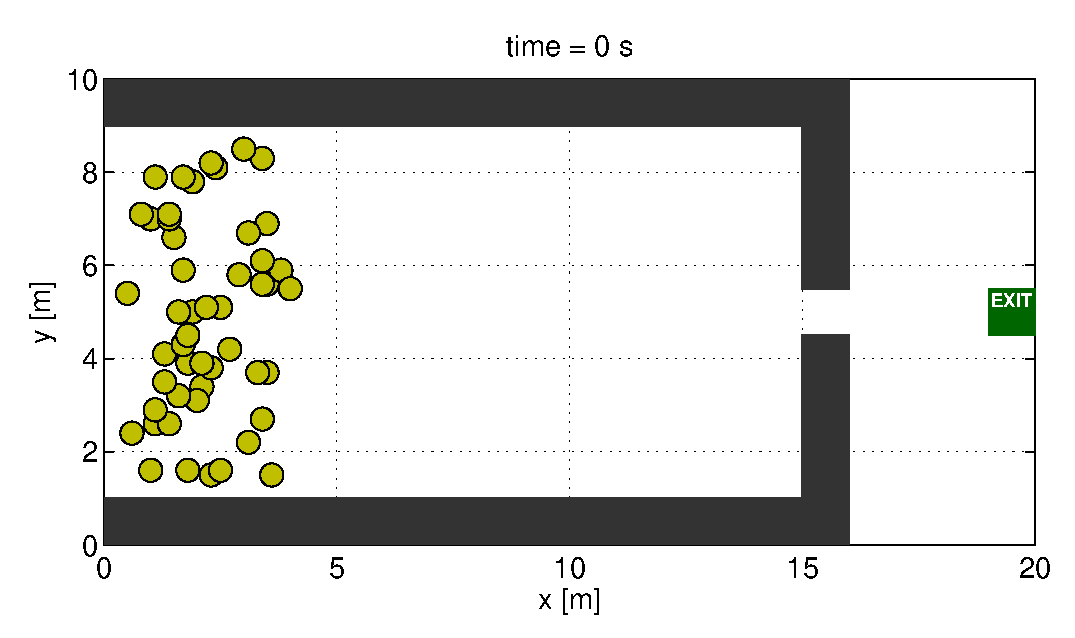
\includegraphics[width=0.7\textwidth]
	{figures/Model1_direct_1b_000000.eps}
	\qquad
	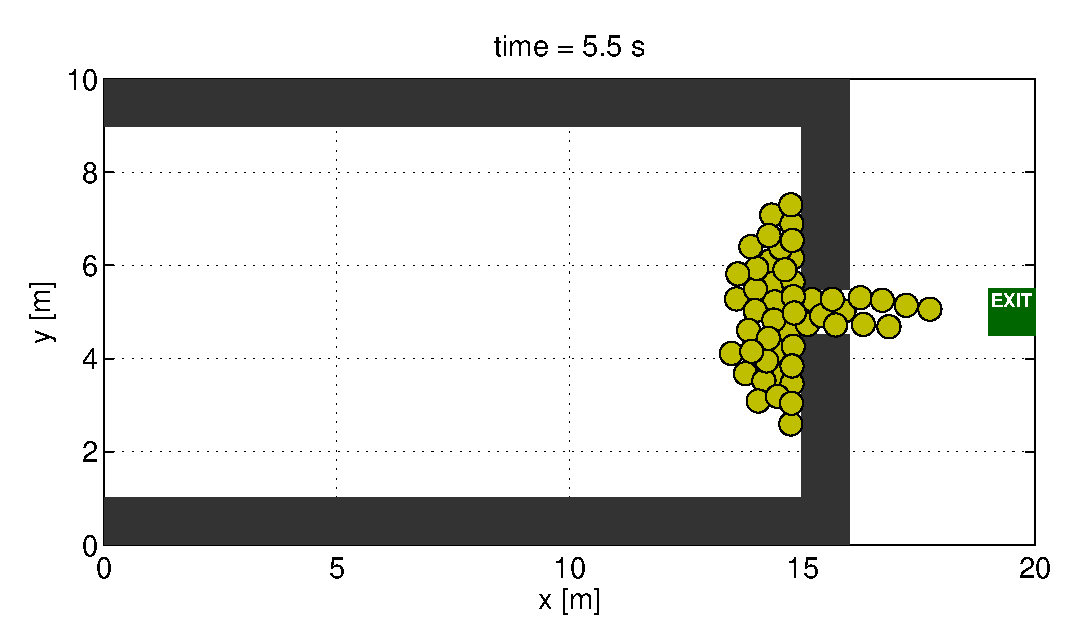
\includegraphics[width=0.7\textwidth]
	{figures/Model1_direct_1b_000550.eps}
	\qquad
	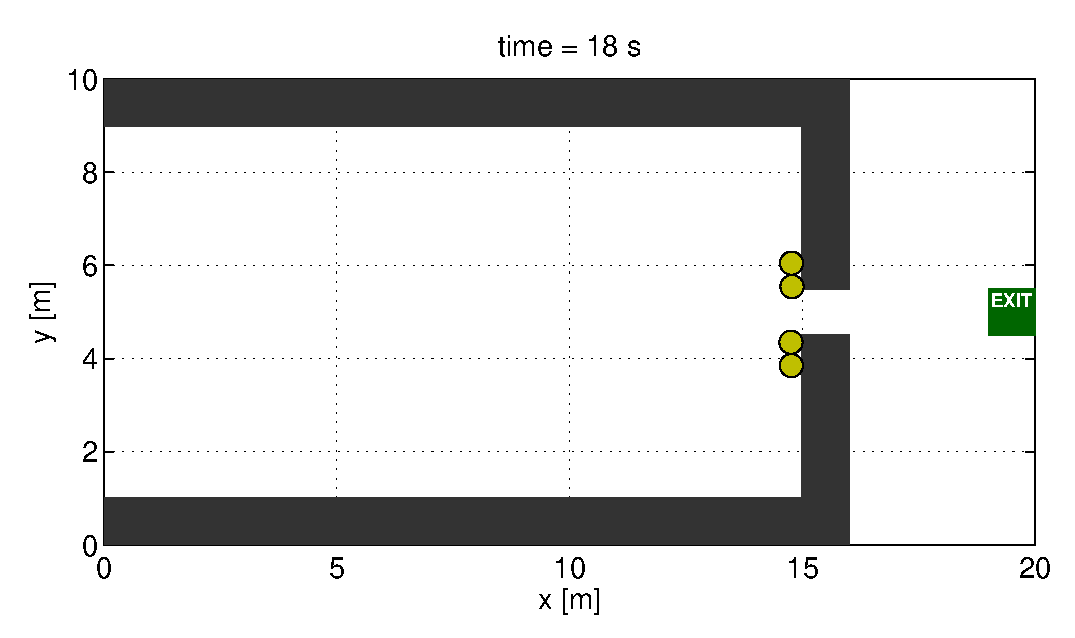
\includegraphics[width=0.7\textwidth]
	{figures/Model1_direct_1b_001800.eps}
	\caption{Simple starting model for a room evacuation through a bottleneck. (a) Initial setup, (b) agents arriving at the bottleneck and accumulating in behind and (c) agents blocking each other of exiting at the end of the simulation.}
	\label{fig:simple1}
	\end{center}
\end{figure}

The simplest version of our code has one exit (Fig.~\ref{fig:simple1}). The attractive force on the agents is defined to be linear towards the exit, thereby neglecting obstacles in between. The agents will not move towards an opening in an obstacle but toward the exit itself. Moreover, this formulation inhibits the agents of running around a bigger obstacle. This is a strong simplification but suitable to test the code. The behavior of the agents towards the repulsive walls and towards each other is satisfactory.

A first case ({\it Model1\_linear\_1}) is shown in Fig.~\ref{fig:simple1}. The model setup consists of a $15\times9$ m room that is bounded by repulsive walls. A $1\times1$ m door is the only exit thereof and leads to the attractive main exit of the model. The agents are initially placed randomly in an $3.5\times7$ m area in the left hand side of the domain (Fig.~\ref{fig:simple1}b). The model is not satisfactory, because at the late stage of evacuation there are two agents opposite of each other preventing them to exit the room (Fig.~\ref{fig:simple1}c). The counter parting psychologic social forces cancel all other forces out and therefore both agents remain at their position.

\begin{figure}
	\begin{center}
	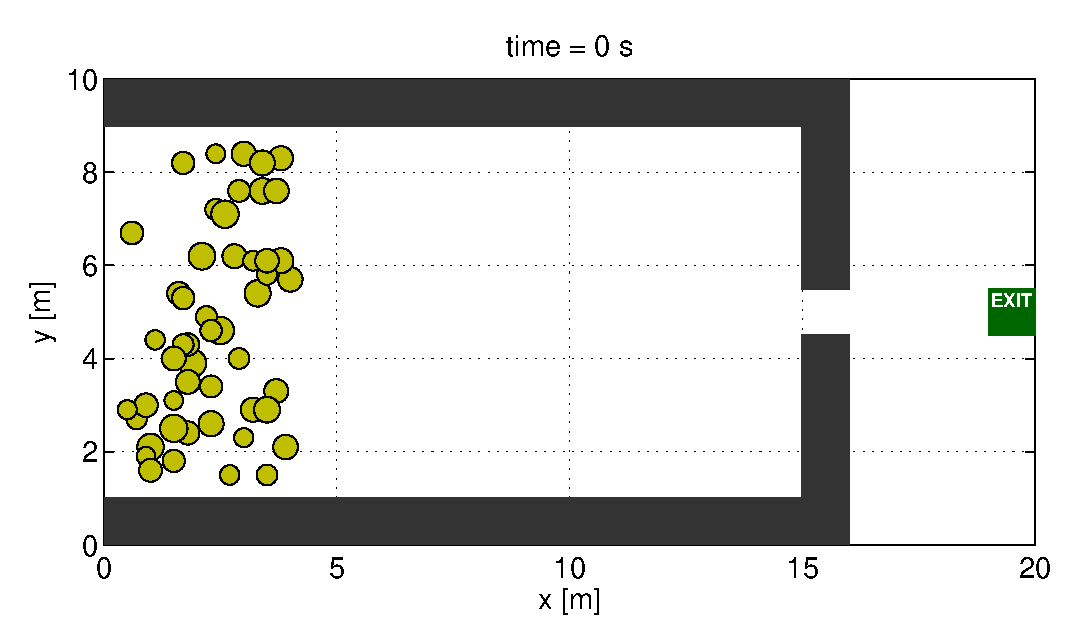
\includegraphics[width=0.7\textwidth]
	{figures/Model1_direct_2b_000000.eps}
	\qquad
	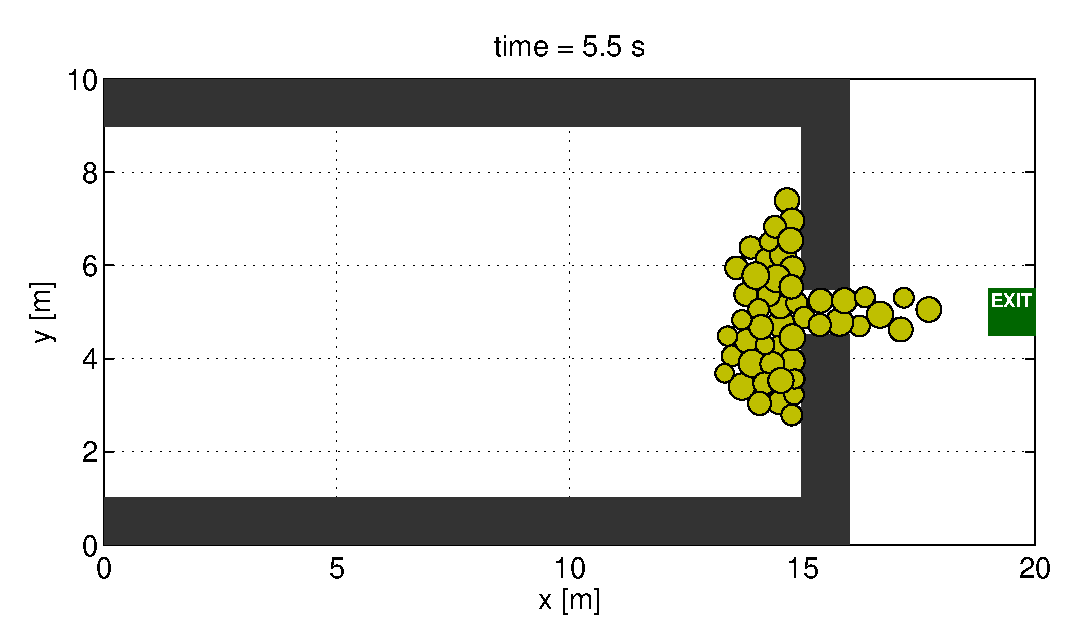
\includegraphics[width=0.7\textwidth]
	{figures/Model1_direct_2b_000550.eps}
	\qquad
	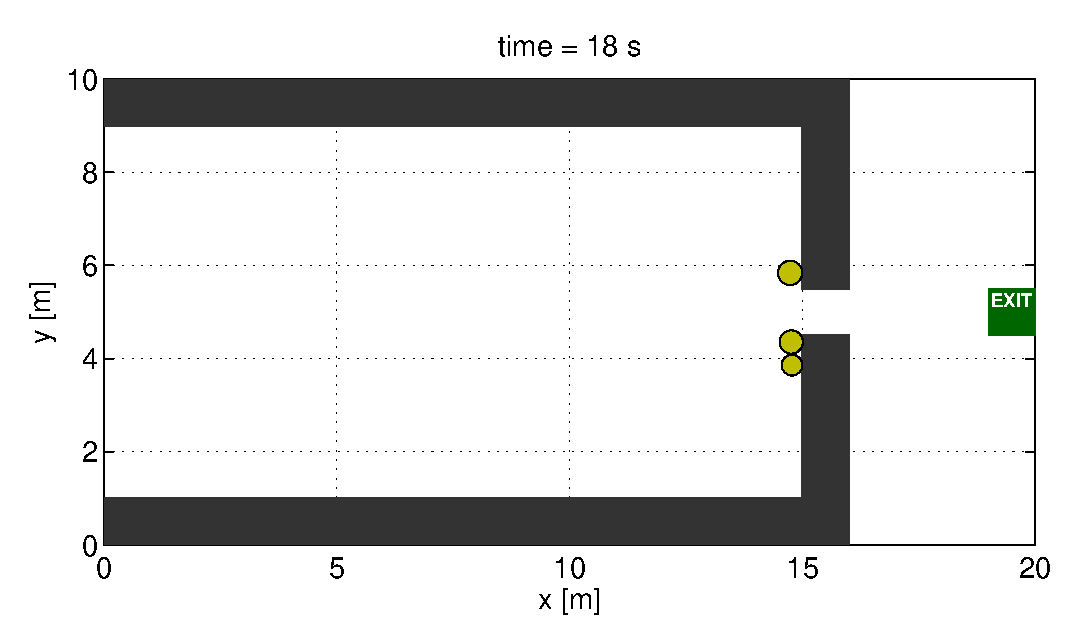
\includegraphics[width=0.7\textwidth]
	{figures/Model1_direct_2b_001800.eps}
	\caption{Model including perturbations for a room evacuation through a bottleneck. (a) Initial setup, (b) agents arriving at the bottleneck and accumulating in behind and (c) agents blocking each other of exiting at the end of the simulation.}
	\label{fig:simple2}
	\end{center}
\end{figure}

In order to introduce some noise into an otherwise perfect model we added several perturbations ({\it Model1\_linear\_2}). The psychologic social force between the agents is perturbed by a random small value in the order of $\pm 0.05$ N. Another complexity is added by characterizing the different agents. Accounting for different appetite and/or stomach behavior, their mass is randomly chosen with a perturbation of $\pm 10$ kg. A bigger radius is subsequently needed for fulfilling mass conservation. Therefore the agent's radius is randomly perturbed by $\pm 0.05$ m. The results of these adjustments are shown in Fig.~\ref{fig:simple2}.

Still the last two pedestrians are disabled of leaving the room because of the counteracting forces they exert on each other. This shows, that the "perfectness" of the model was not the main problem of this occurrence. The main cause of it might be found in the way the attractive exit force is described. The agents are pulled with the exit force directly towards the position of the exit, neglecting possible obstacles in between. Hence, in the case of the two blocked pedestrians, the main force is directed perpendicular to the wall instead of tangential to the wall towards the wall door. The force in this direction is very small and can thus easily be overweighted by the repulsive social force of the opposite agent. The agent is kept at his current position.

A solution of this problem therefore might be found in a different description of the attractive exit force by e.g. using a shortest path formulation.

\subsubsection{Shortest path formulation}

The shortest path formulation as described in Section~\ref{sec:Exits1} can improve the nature-like behavior of the model dramatically. A new setup is chosen to illustrate this and shown in Fig.~\ref{fig:simple3} and~\ref{fig:simple4}.

\begin{figure}
	\begin{center}
	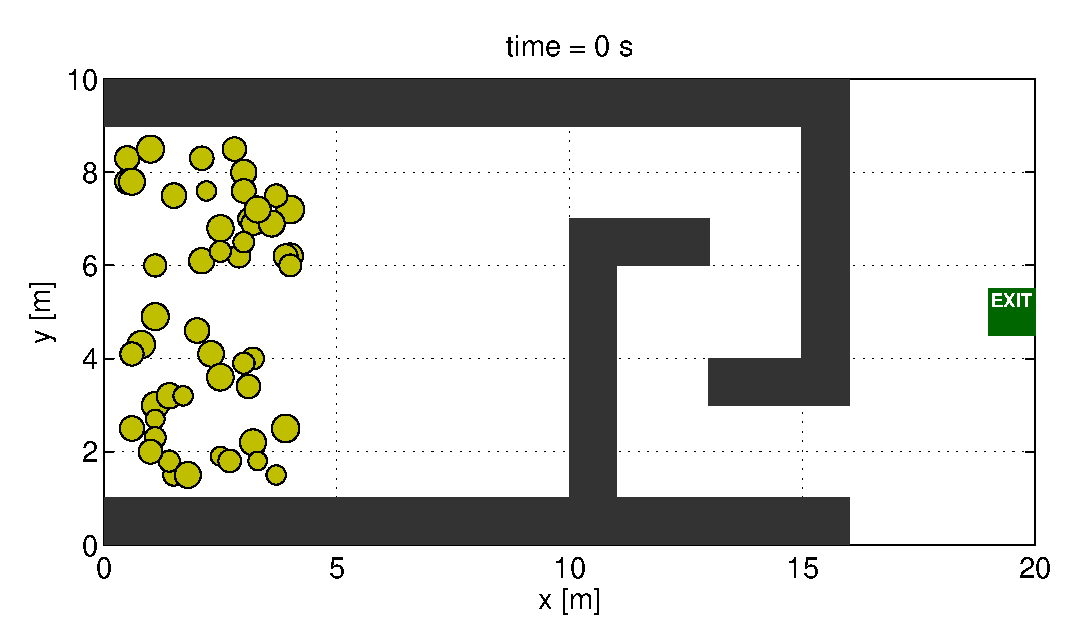
\includegraphics[width=0.7\textwidth]
	{figures/Model2_direct_1b_000000.eps}
	\qquad
	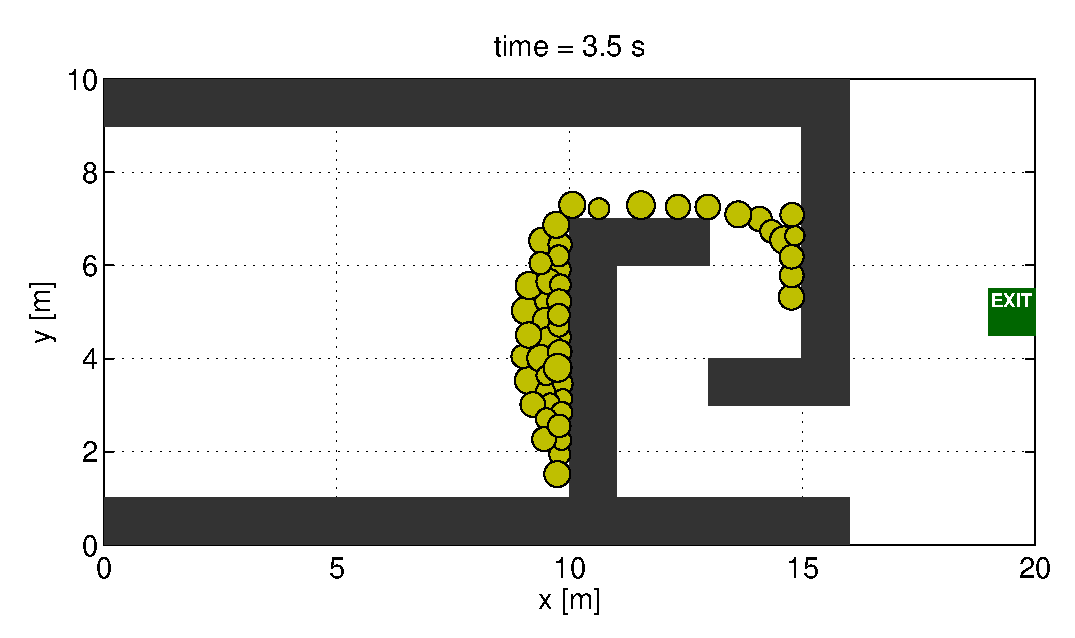
\includegraphics[width=0.7\textwidth]
	{figures/Model2_direct_1b_000350.eps}
	\qquad
	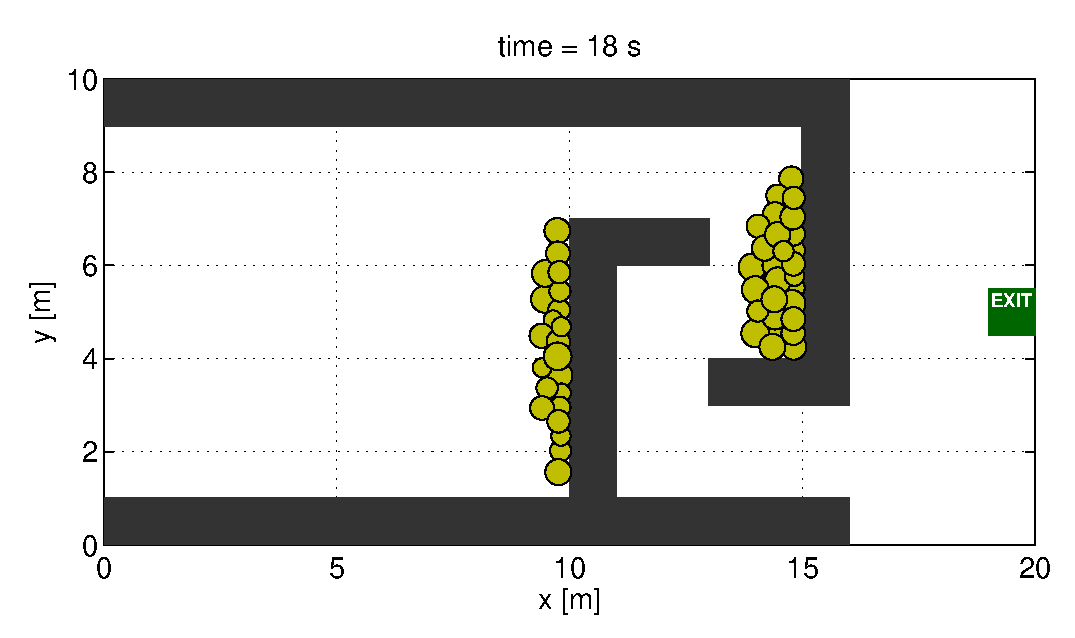
\includegraphics[width=0.7\textwidth]
	{figures/Model2_direct_1b_001800.eps}
	\caption{Model with direct exit force formulation for a pedestrian flow around complicated architecture. (a) Initial setup, (b) agents arriving at the barrier walls and accumulating and (c) agents getting stuck and not able to move around an obstacle at the end of the simulation.}
	\label{fig:simple3}
	\end{center}
\end{figure}

The walls are placed in a way that the pedestrians have to move around corners and even away from the exit to finally arrive there. This is not straight forward and a simple exit force formulation is not able to describe the pedestrian flow in such a case (Fig.~\ref{fig:simple3}). The Agents get captured by obstacles with no direct passage towards the exit and are not able to leave such a place. 

The more elaborated shortest path formulation, on the other hand, can describe such a more complicated pedestrian flow in a realistic manner (Fig.~\ref{fig:simple4}). The agents are able to see all possible passages towards an exit in the whole model and are therefore able to choose the fastest way.

\begin{figure}
	\begin{center}
	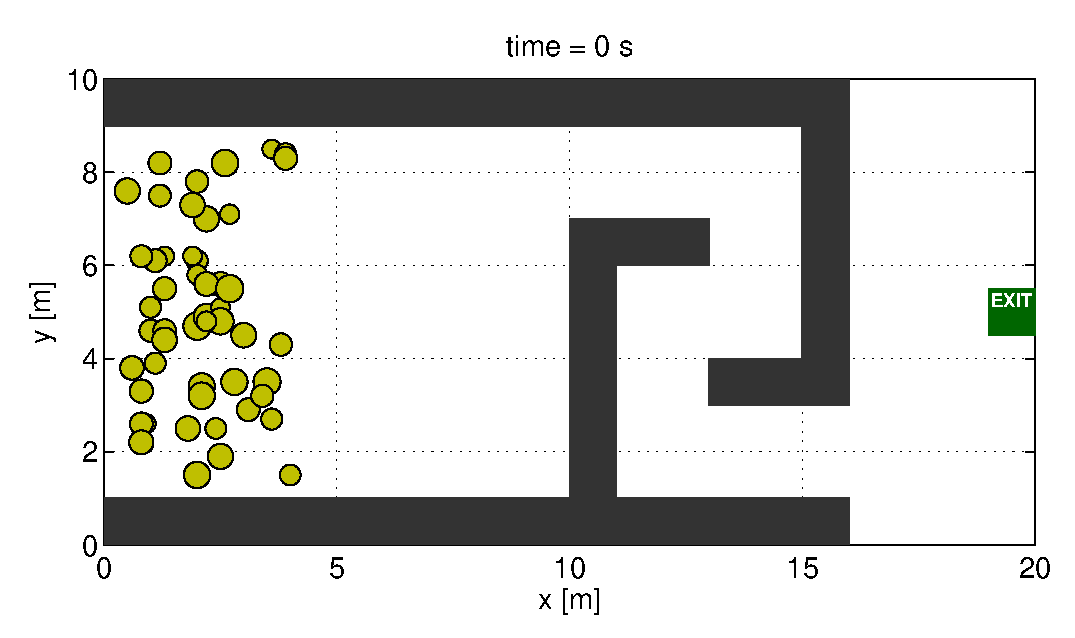
\includegraphics[width=0.7\textwidth]
	{figures/Model2_fastest_1_000000.eps}
	\qquad
	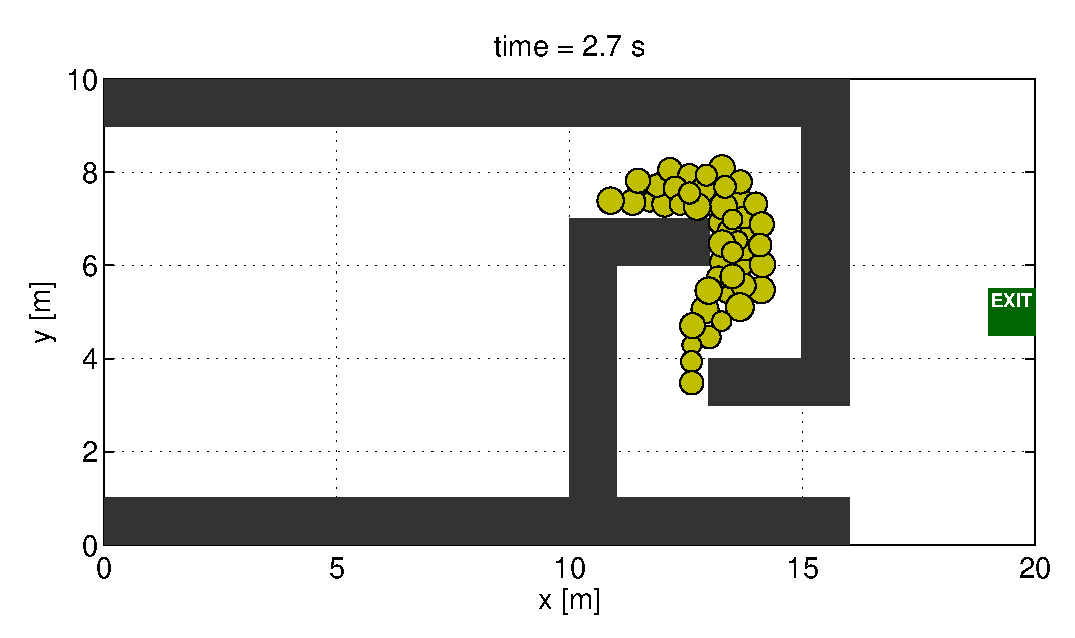
\includegraphics[width=0.7\textwidth]
	{figures/Model2_fastest_1_000270.eps}
	\qquad
	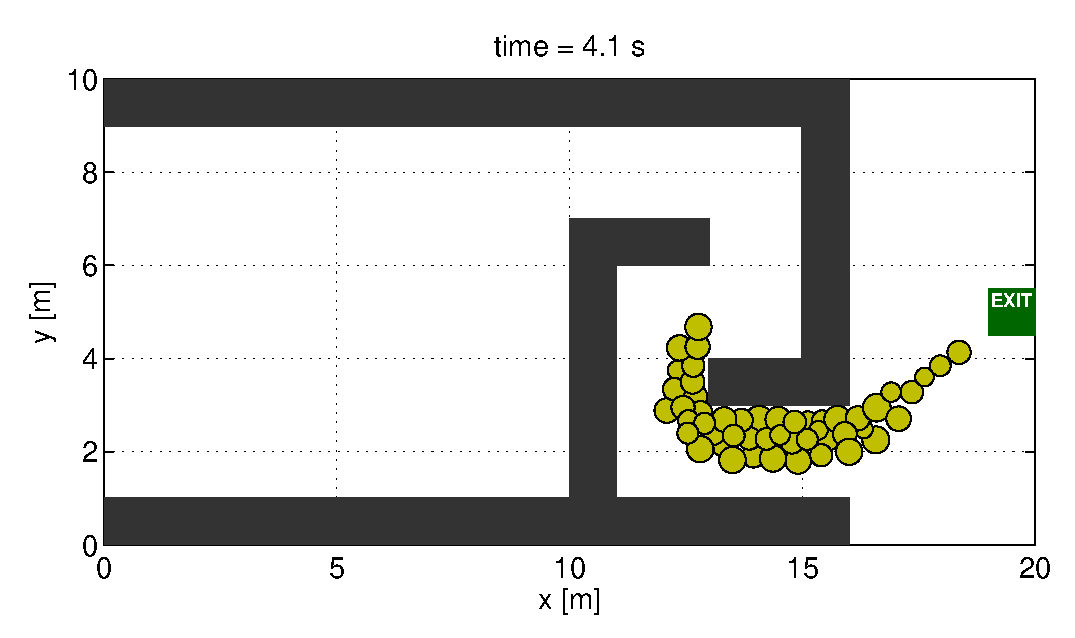
\includegraphics[width=0.7\textwidth]
	{figures/Model2_fastest_1_000410.eps}
	\caption{Model including shortest path formulation for a pedestrian flow around complicated architecture. (a) Initial setup, (b) agents moving closely around corners and (c) agents able to move around obstacles in the fastest way and arriving the exit at the end of the simulation.}
	\label{fig:simple4}
	\end{center}
\end{figure}

\subsection{Simple evacuation bottleneck: Two exits}

As we saw in the one-exit models, the shortest path formalism led to a more realistic behaviour of the agents. In a second step, we now extended the model by introducing one additional exit, leaving out the additional obstacles. In a first step, we used the shortest path procedure to determine the desired direction of the agent. As this did not lead to the desired agent behaviour (see Section~\ref{sec:two_exits1}), we had to extend the shortest path procedure by additionally taking agents into account (the procedure is described in Section~\ref{sec:implementation}). This led to a significant improvement in agent behaviour. As we additionally have to deal with topography in our model, we then introduced a small topography in our model to assess its effect on agent behaviour. In the three following subsection, we shortly show and discuss the results of the different setups.

\subsubsection{Shortest path exit force}\label{sec:two_exits1}

Here, the exit direction of the agents is given by the shortest path algorithm, which has proven to yield better results compared to the direct path approach. Instead of having one gap in the wall as before, we now have two gaps in the wall. Additionally, the exit was switched slightly towards the lower gap. This makes the lower gap more preferable, since the path to the exit through this gap is shorter.

As one can see in Fig.~\ref{fig:two_exits1}, the shortest path algorithm results in a rather unrealistic behaviour of the agents: Instead of opting for the upper gap in case the lower gap is blocked by other agents, all agents choose the lower gap.

\begin{figure}
	\centering
	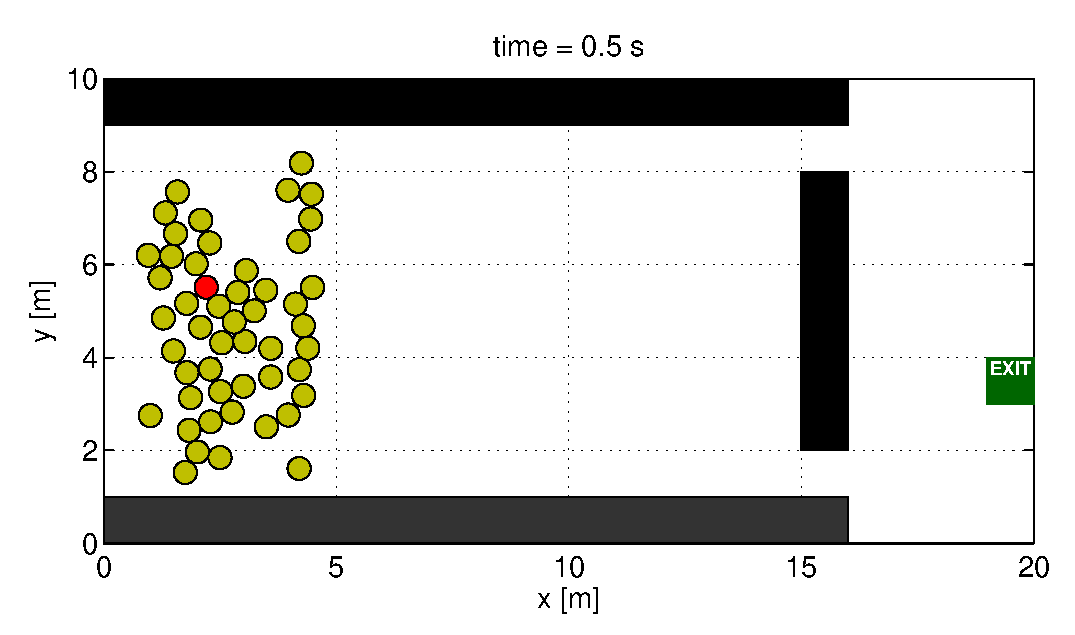
\includegraphics[width=0.6\textwidth]{figures/TwoExitsShortestPath_000050.eps}
	\qquad
	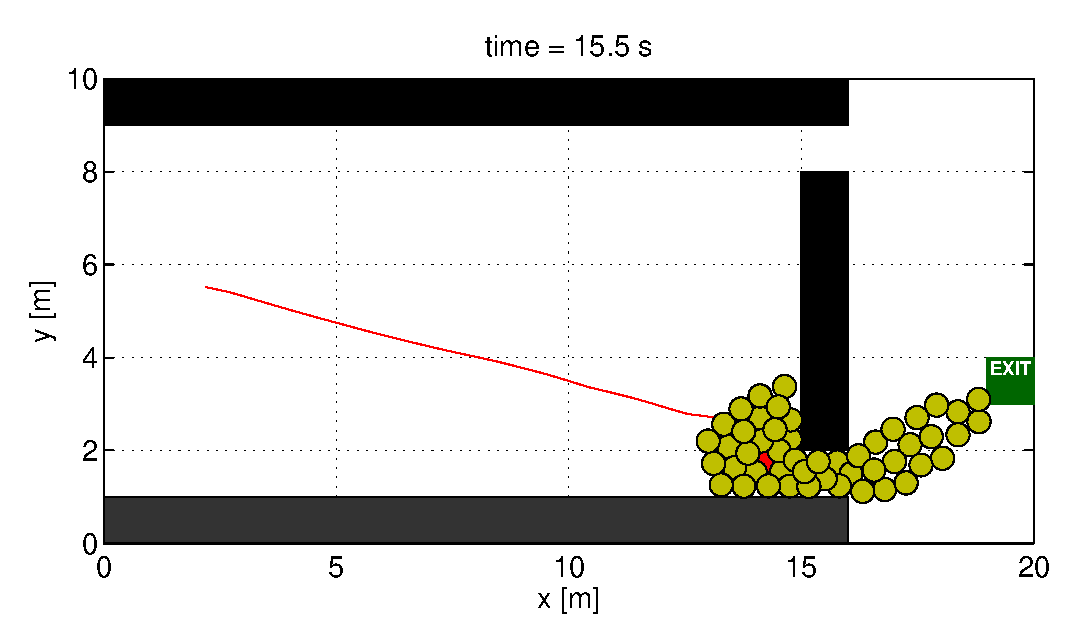
\includegraphics[width=0.6\textwidth]{figures/TwoExitsShortestPath_001550.eps}
	\qquad
	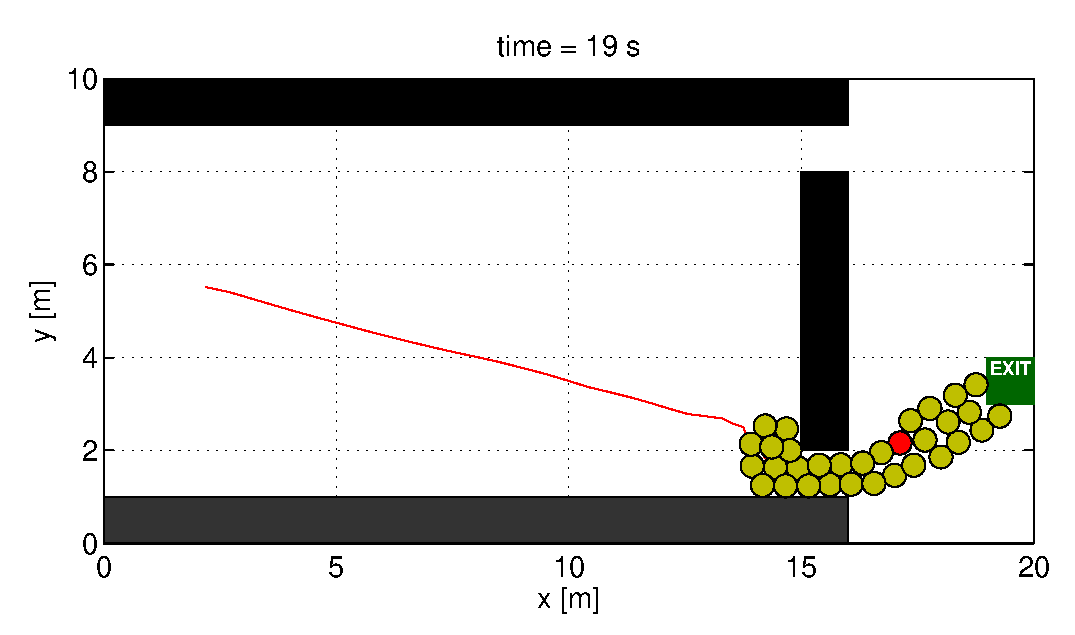
\includegraphics[width=0.6\textwidth]{figures/TwoExitsShortestPath_001900.eps}
	\caption{Snapshots of the time evolution of a simple two-exit model using the shortest path algorithm to determine the exit direction. As can be seen, the simple shortest path formalism doesn't work in a realistic manner, since all the agents opt for the closest exit regardless of other agents blocking the way. For a better illustration, we chose one agent (named Don) and plot his path through the model domain. As one can see, Don never changes his direction on the way to the exit.}
	\label{fig:two_exits1}
\end{figure}

This behaviour is clearly not what one could observe in reality, since at least some agents would prefer the upper gap and reach the exit significantly faster than in our simulation. We therefore had to adjust the shortest path procedure to account for agents blocking the way.
\subsubsection{Shortest path exit force with agents taken into account}
In the second simulation, we used the extended shortest path procedure to determine the exit direction of the agents. We tried different combinations of the sensitivity of the agents to other agents blocking the way. The (in our opinion) best results were obtained when we reduced the estimated velocity at a node by a factor of 2.5. In Fig.~\ref{fig:two_exits2}, it can be seen that the behaviour of the agents is much more realistic than before. In this simulation, agents frequently re-decide on the path to be taken and change from the lower to the upper gap or vice versa if either of those gaps is blocked.

\begin{figure}
	\centering
	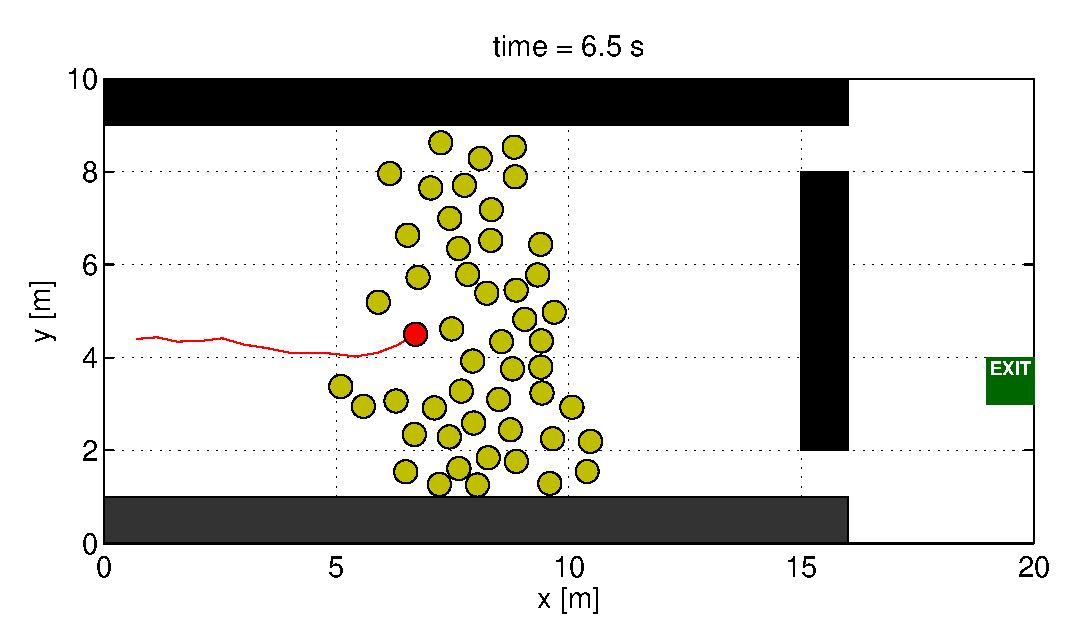
\includegraphics[width=0.6\textwidth]{figures/TwoExitsShortestPathWithAgents_000650.eps}
	\qquad
	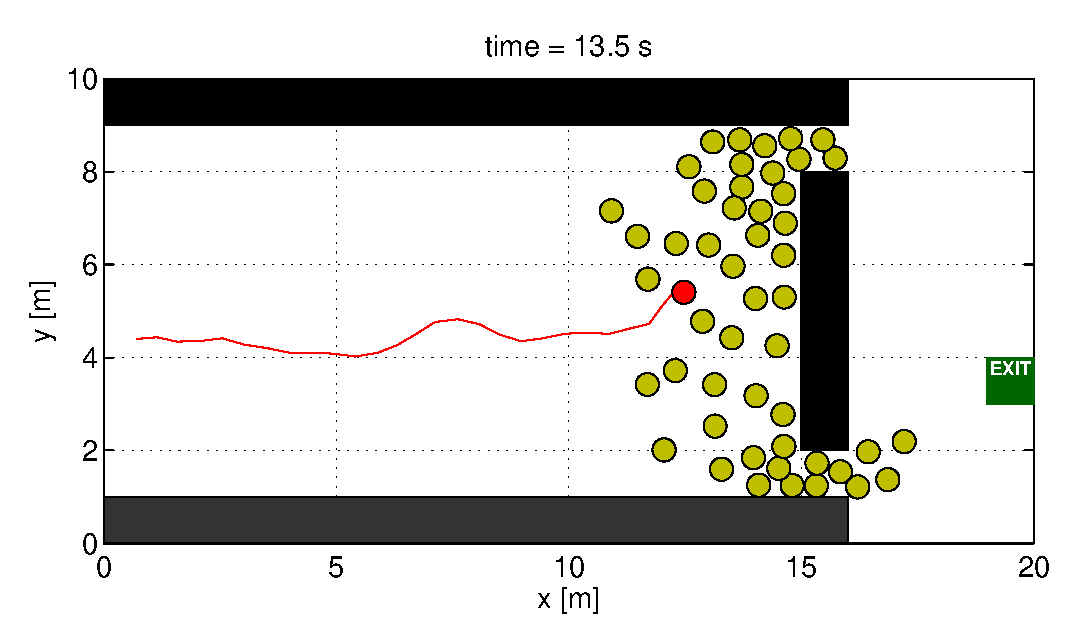
\includegraphics[width=0.6\textwidth]{figures/TwoExitsShortestPathWithAgents_001350.eps}
	\qquad
	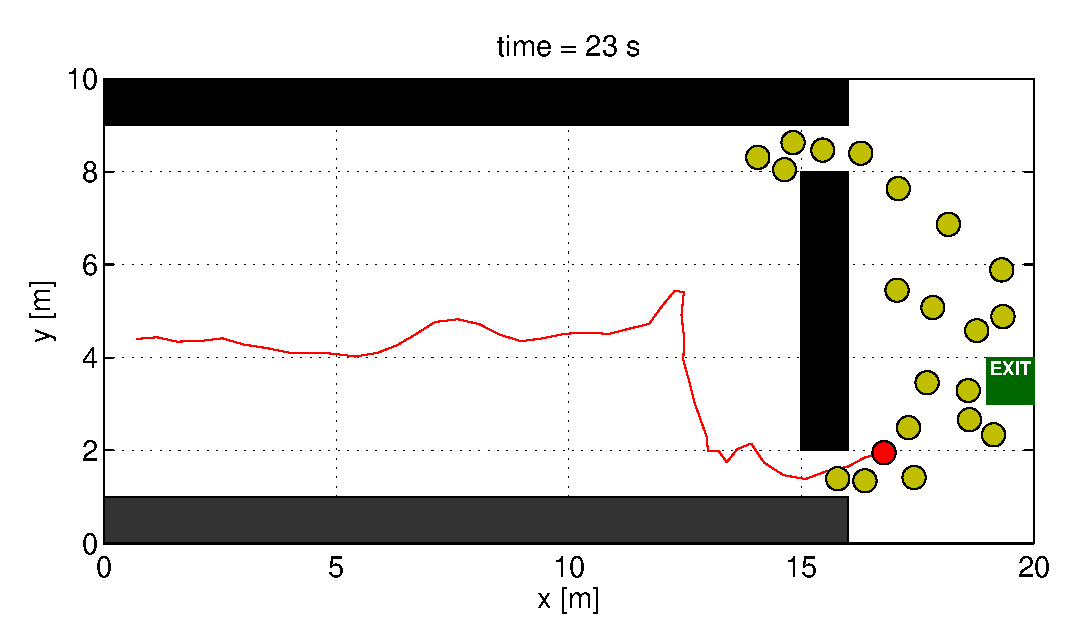
\includegraphics[width=0.6\textwidth]{figures/TwoExitsShortestPathWithAgents_002300.eps}
	\caption{Snapshots of the time evolution of a simple two-exit model using the shortest path algorithm to determine the exit direction. In this case, agents blocking the way to the exit are taken into account. This enables the agents to redecide on the path taken to the exit depending on the agent density in between. The path of our example agent Don clearly shows this process. At first, Don chooses a path that keeps him in between both exits due to the agents in front of him. Then, as crowding at the lower exit occurs, he decides to go towards the upper exit, but then redecides as the lower exit becomes less crowded again.}
	\label{fig:two_exits2}
\end{figure}

\subsubsection{Shortest path exit force with agents and topography taken into account}

In this last simulation, we tested the influence of topography on agent behaviour. For this reason, we introduced a slight topography in our model. The topography is essentially a two-dimensional Gaussian curve, which is given by the equation:

\begin{equation}
	z(x,y) = A\exp \left(- \frac{\left(x-x_0\right)^2}{2\sigma_x} + \frac{\left(y-y_0\right)^2}{2\sigma_y}\right)
\end{equation}

In this simulation, we chose $A = 1 $ m, $x_0 = 10$ m, $y_0 = 5$ m, $\sigma_x = 15$ m and $\sigma_y = 6$ m.


\subsection{Evacuation through a road network}

\subsection{Evacuation through a road network with topography and flooding}

\subsection{Evacuation of a beach in the case of a tsunami event}

\begin{figure}
	\centering
	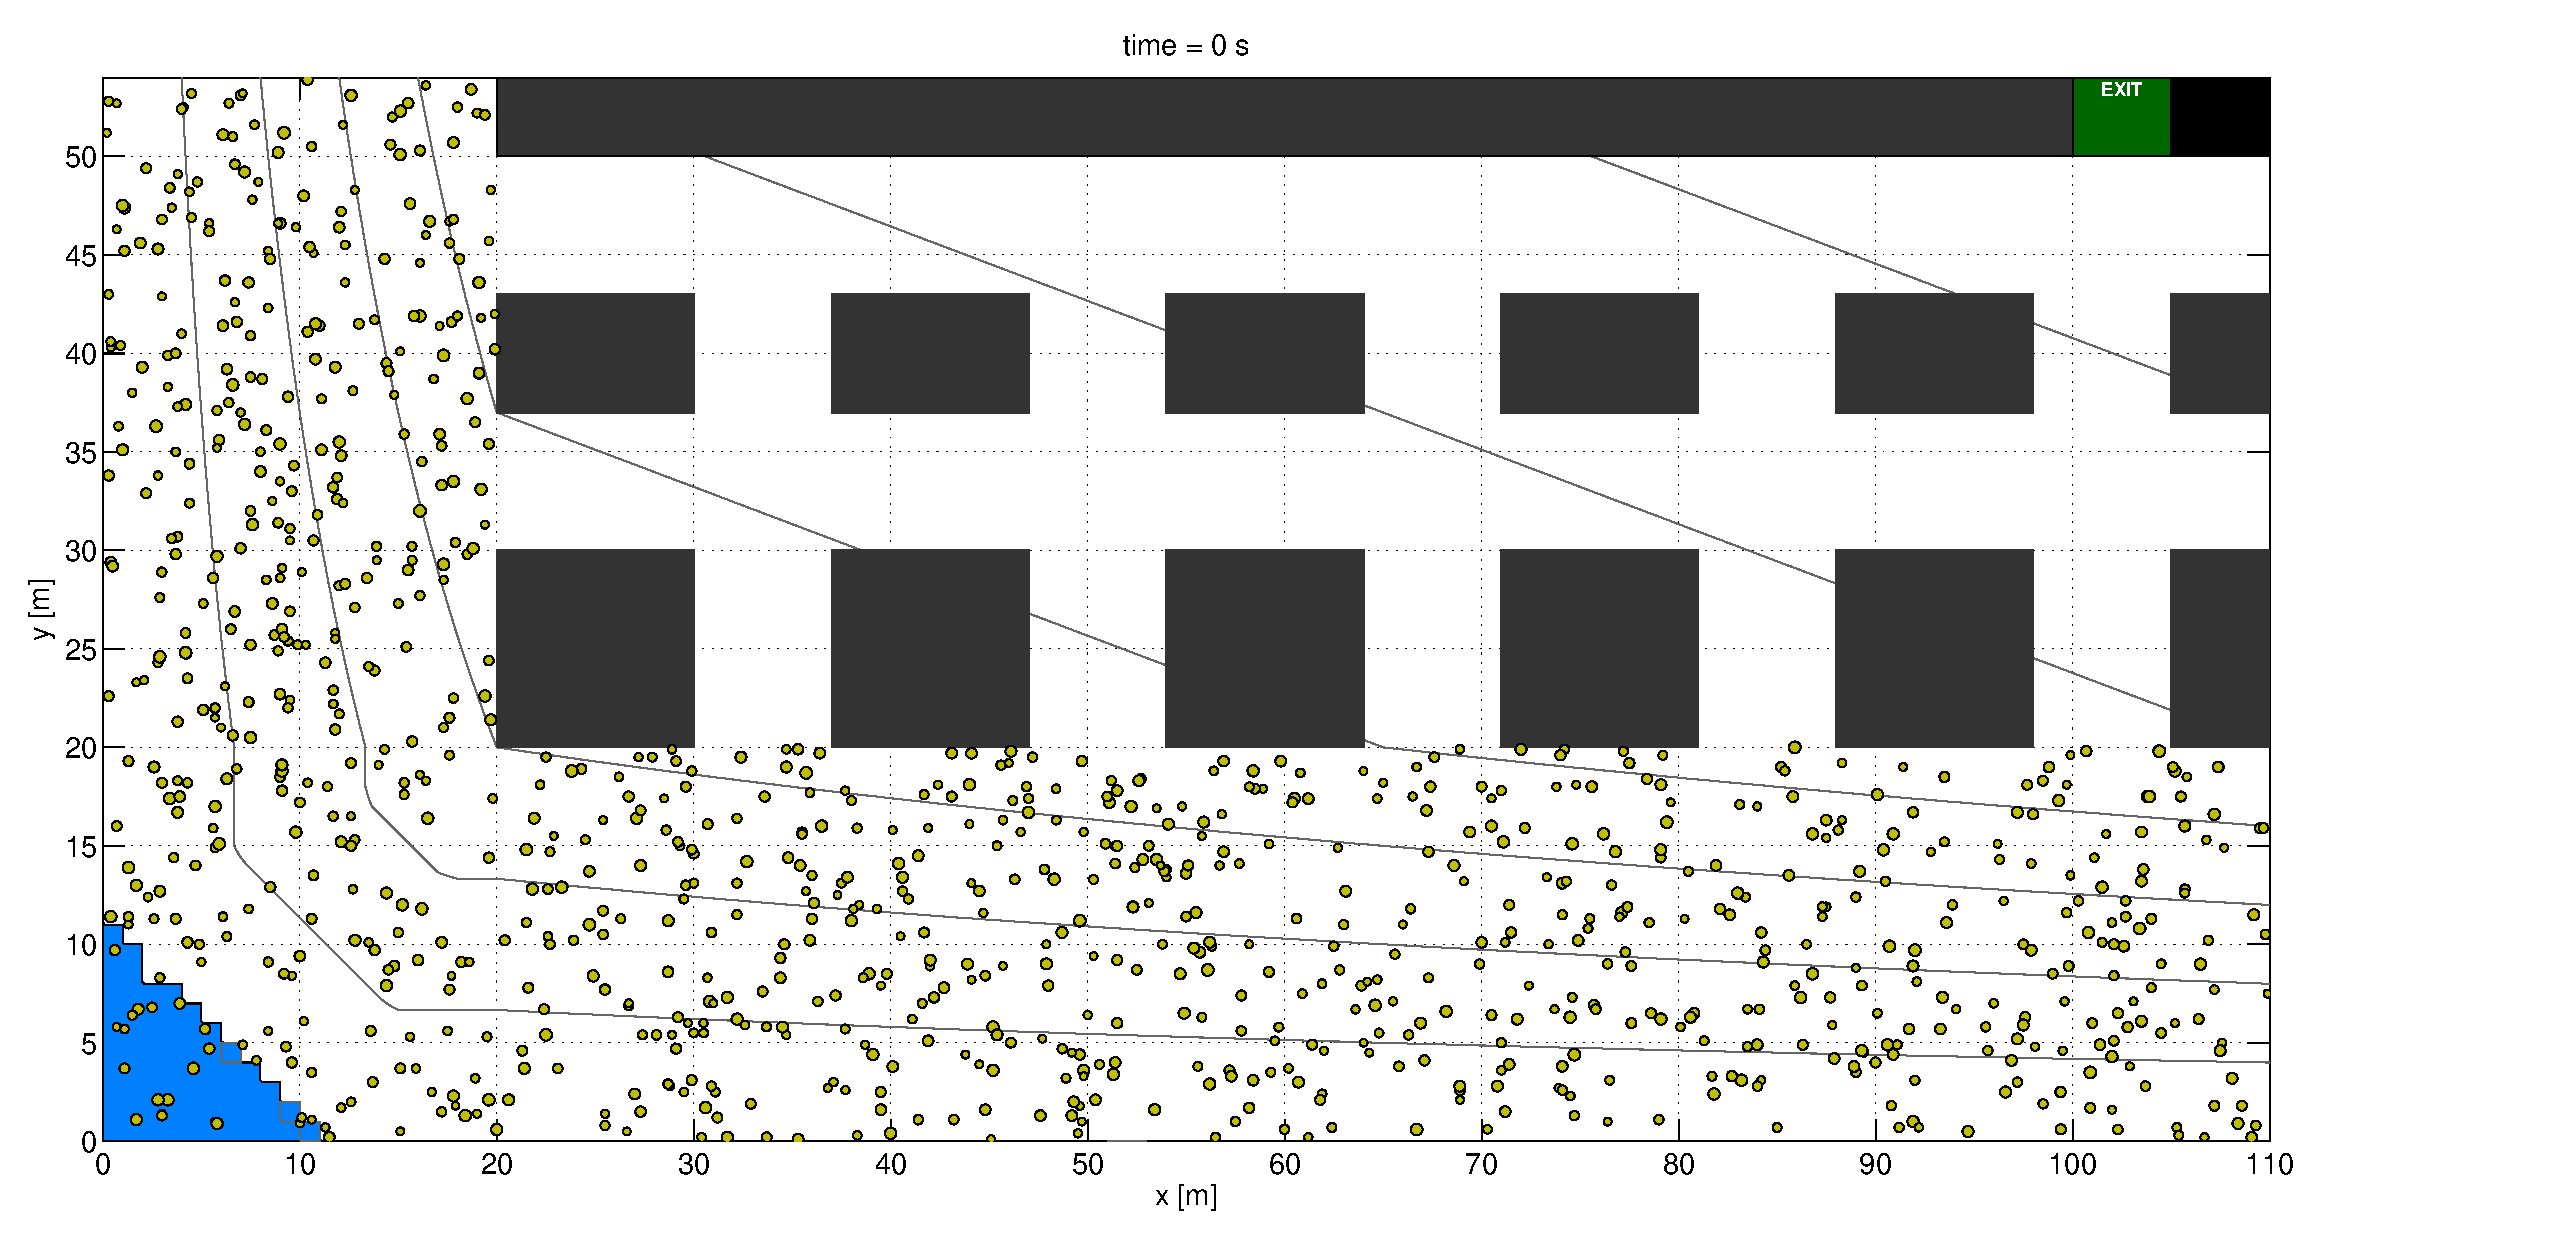
\includegraphics[width=1.1\textwidth]{figures/BeachEvacuationOneExitStreetWidth7_Flood0_1_000000.eps}
		\qquad
	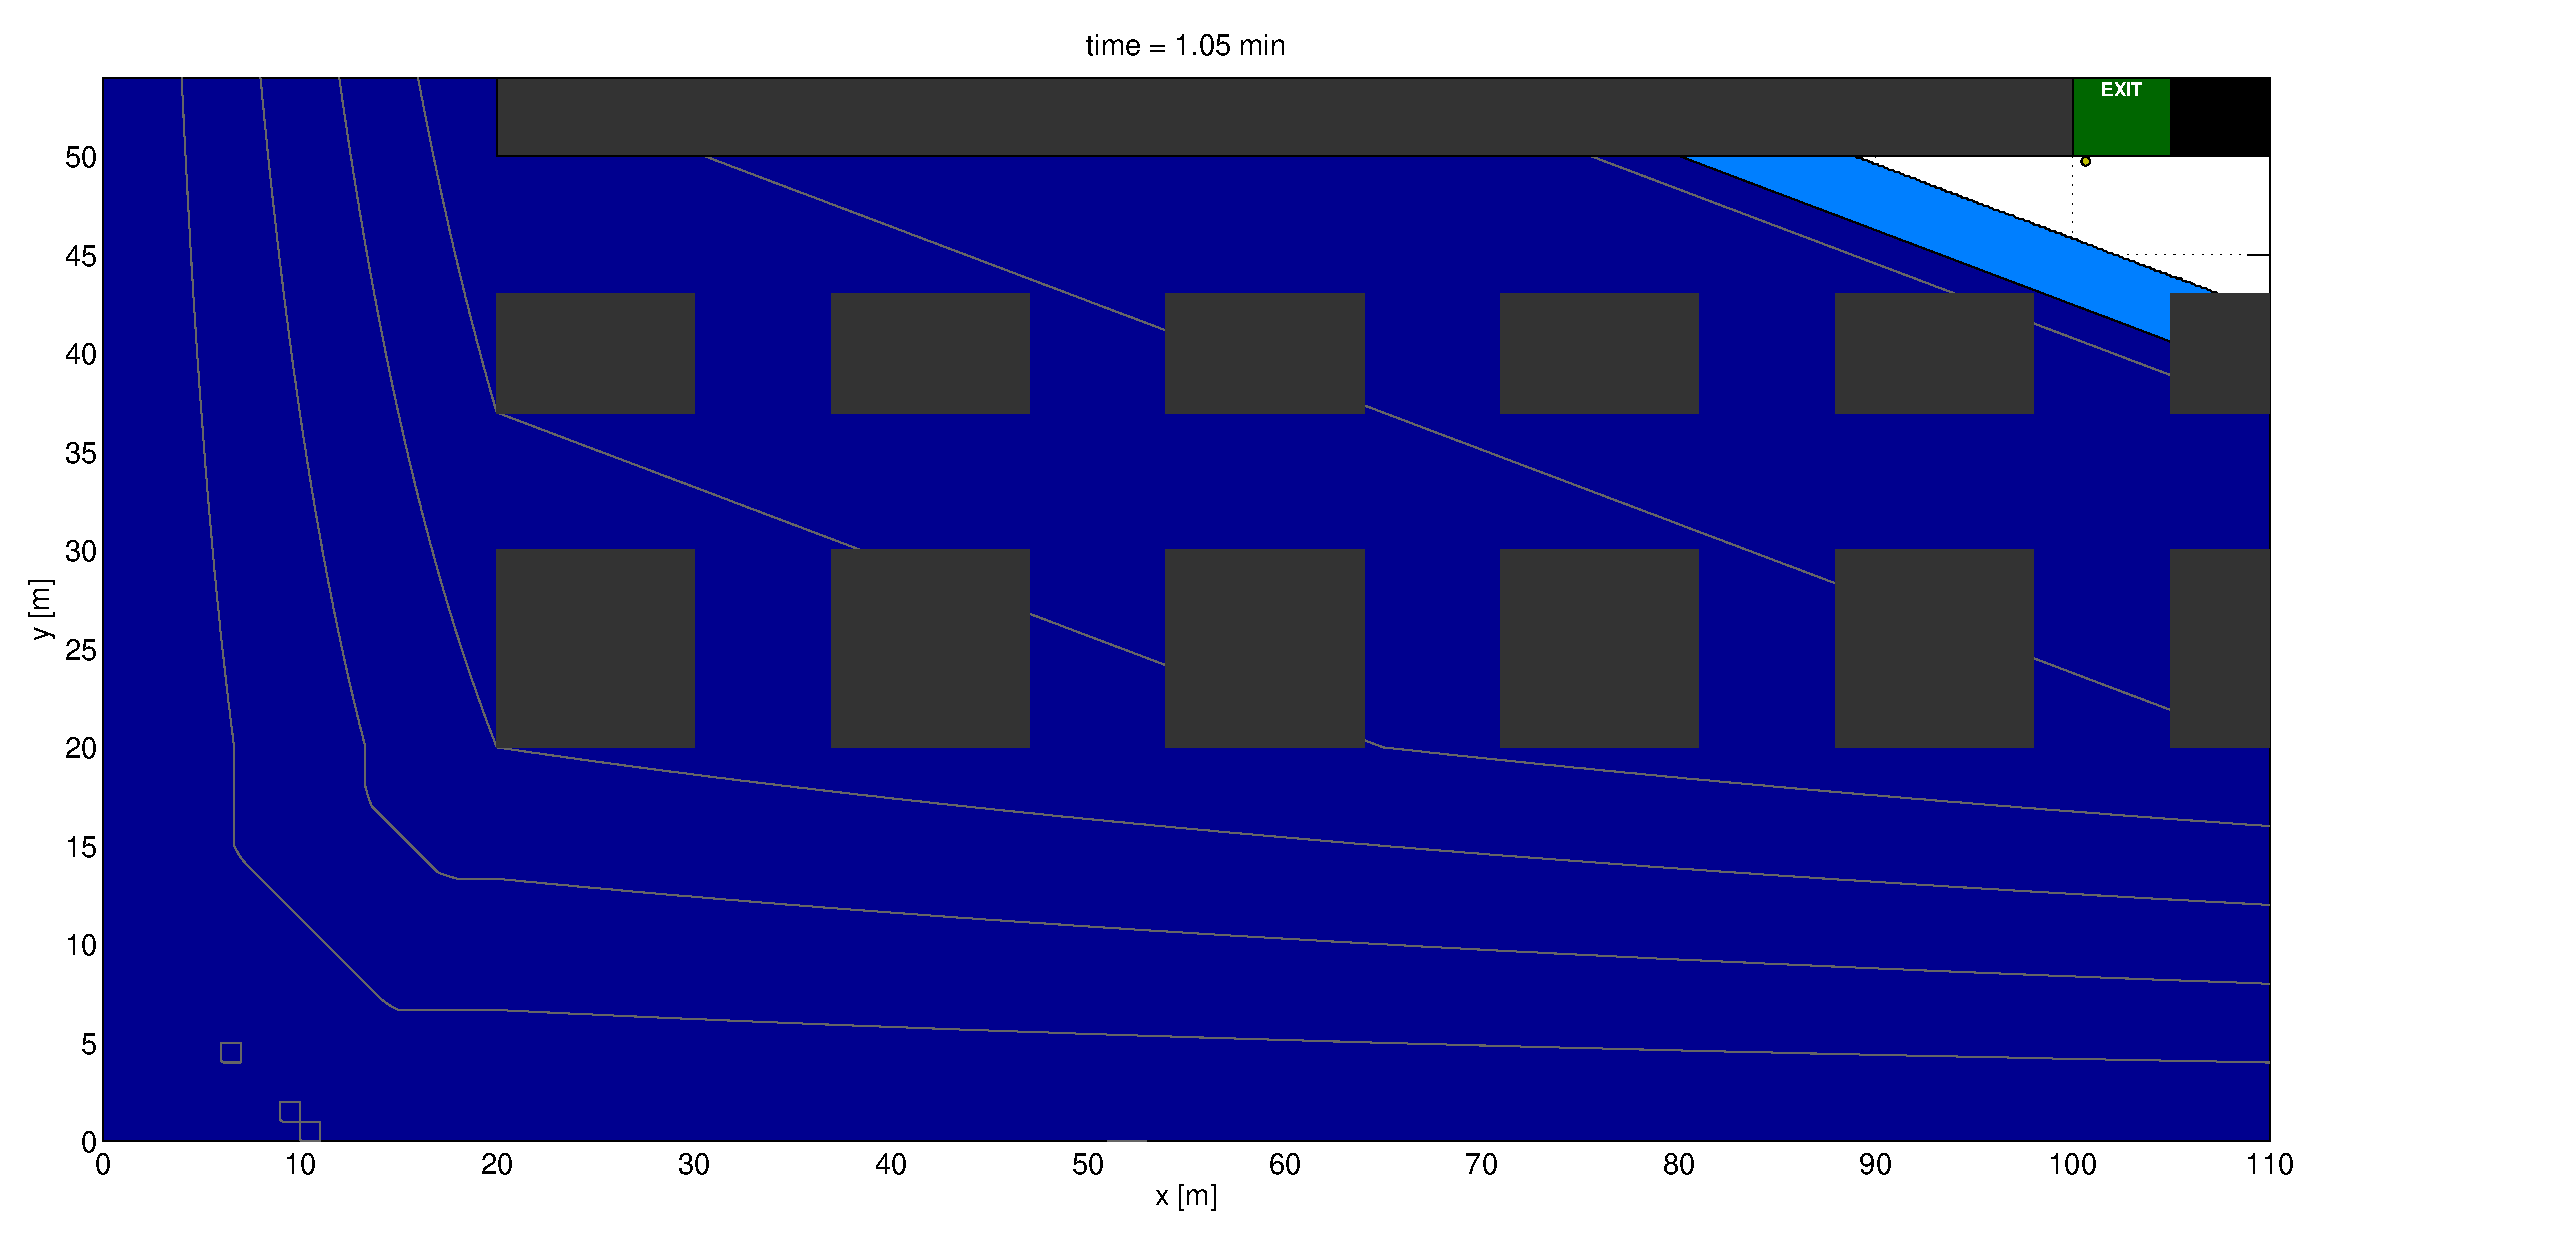
\includegraphics[width=1.1\textwidth]{figures/BeachEvacuationOneExitStreetWidth7_Flood0_1_006300.eps}
	\caption{Initial condition of the beach evacuation model: 1000 pedestrians (yellow circles) swimming or lying in the sun (top). Final stage of evacuation model: last surviving pedestrian arrives at exit just before the flood reaches him. Black squares indicating beach houses or anti-flood wall, green square is the exit, grey contours indicating topography and blue contour indicates water covered surface.}
	\label{fig:beach_initial}
\end{figure}

\begin{figure}
	\centering
	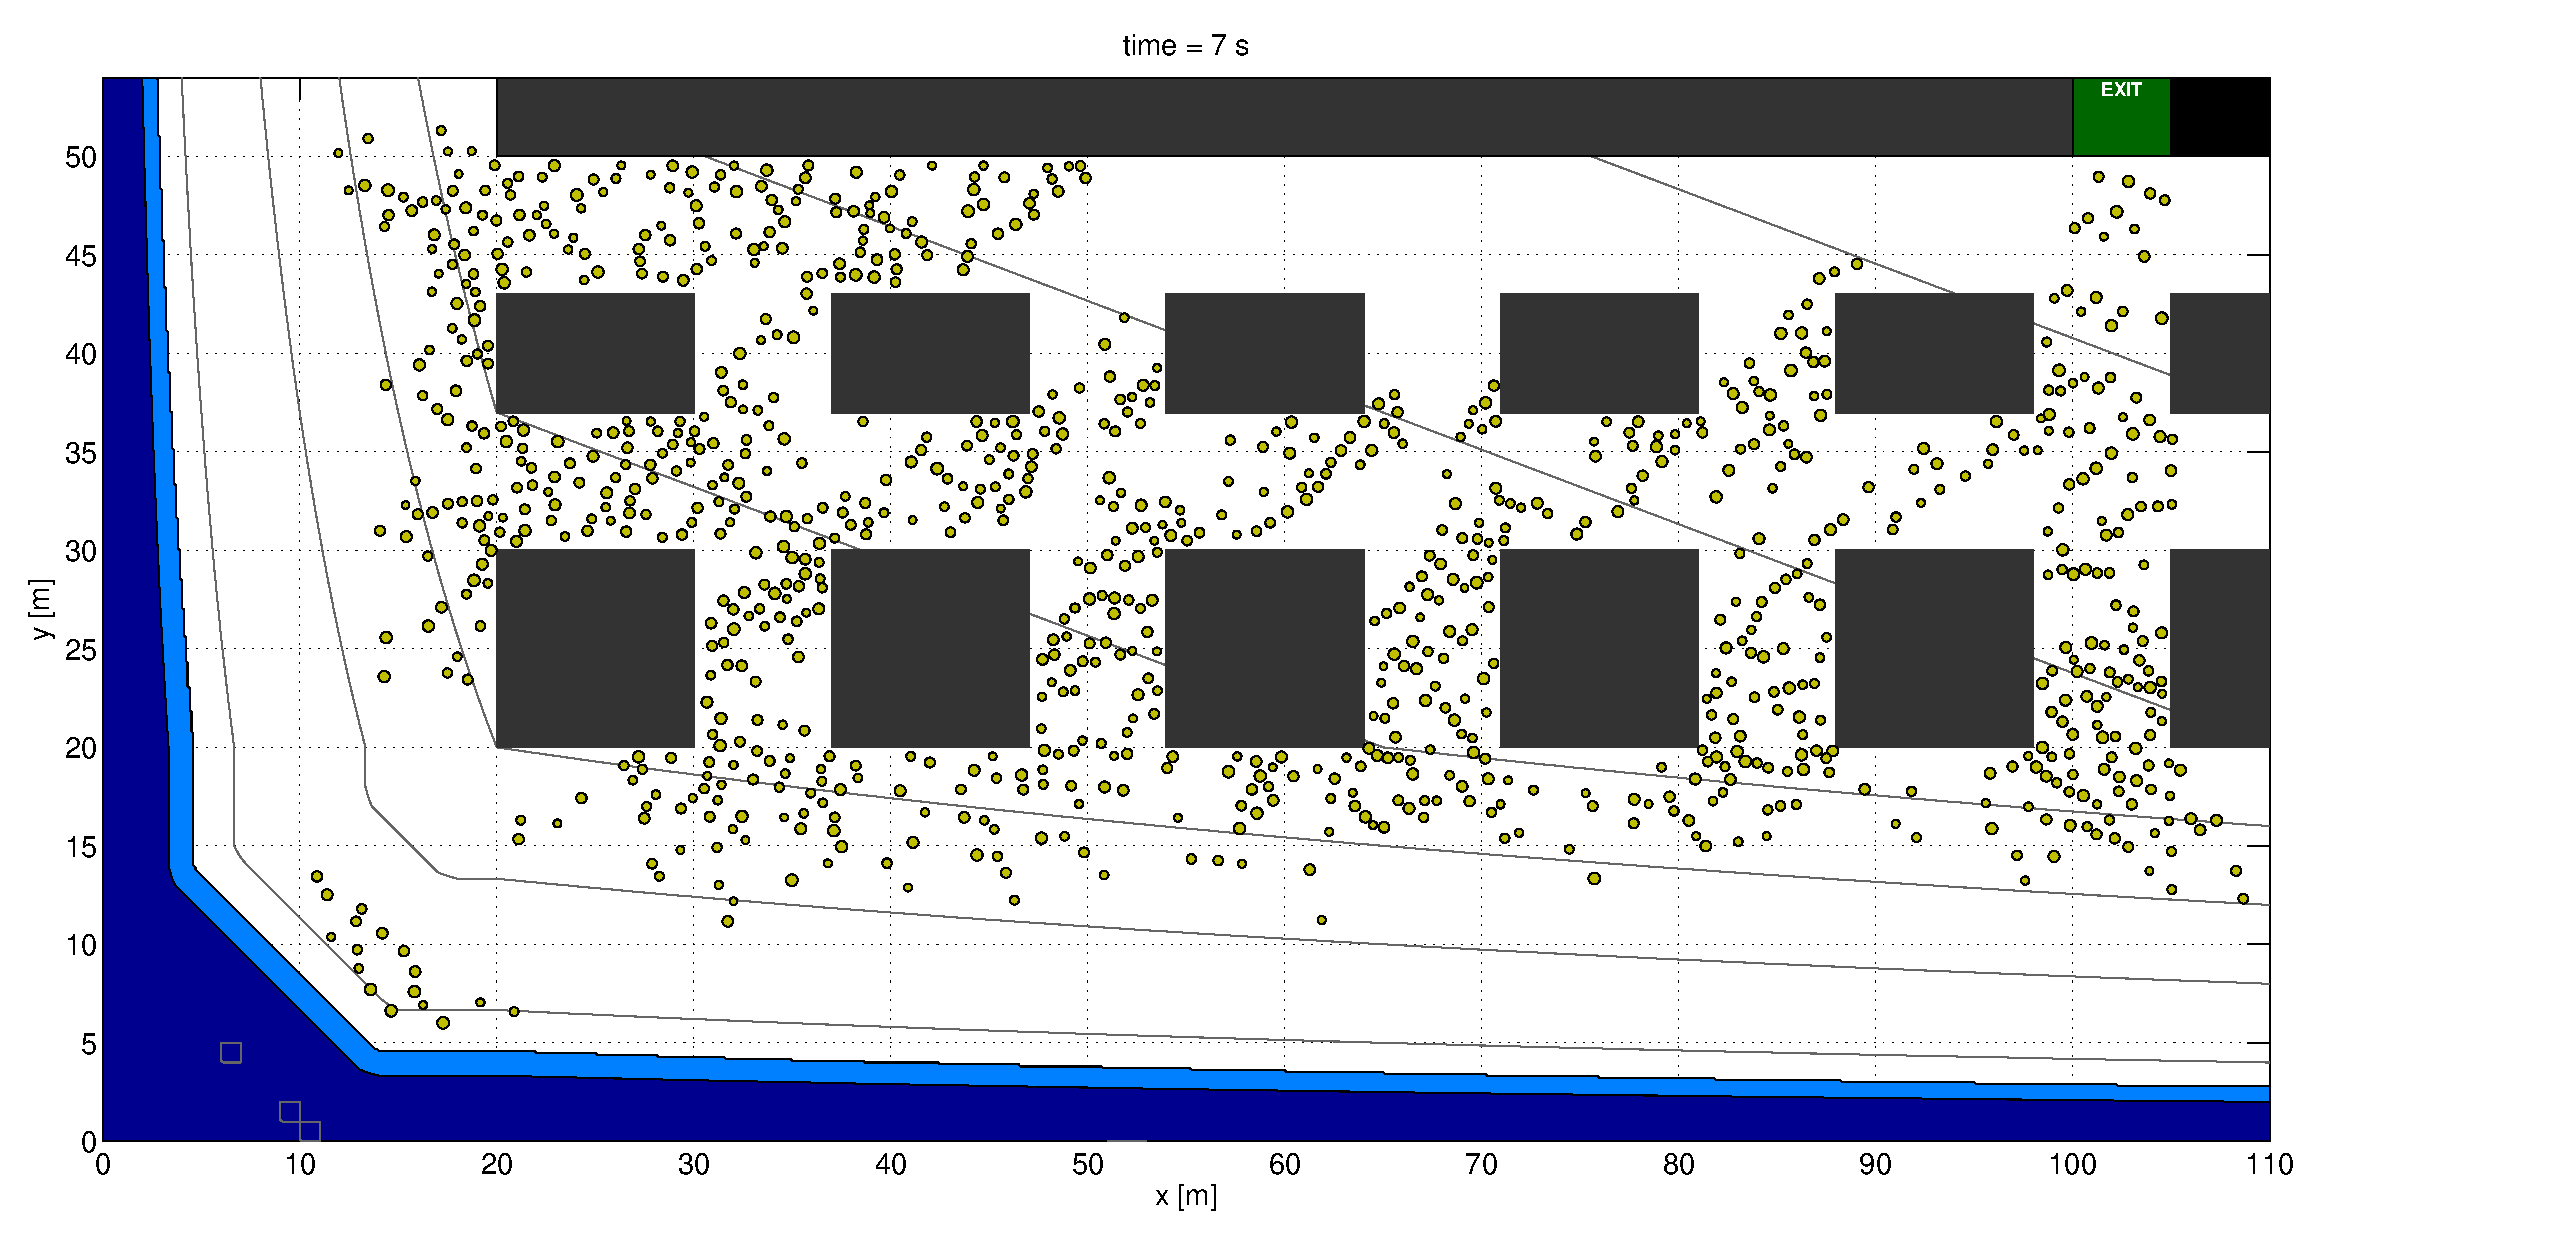
\includegraphics[width=1.1\textwidth]{figures/BeachEvacuationOneExitStreetWidth7_Flood0_1_000700.eps}
	\qquad
	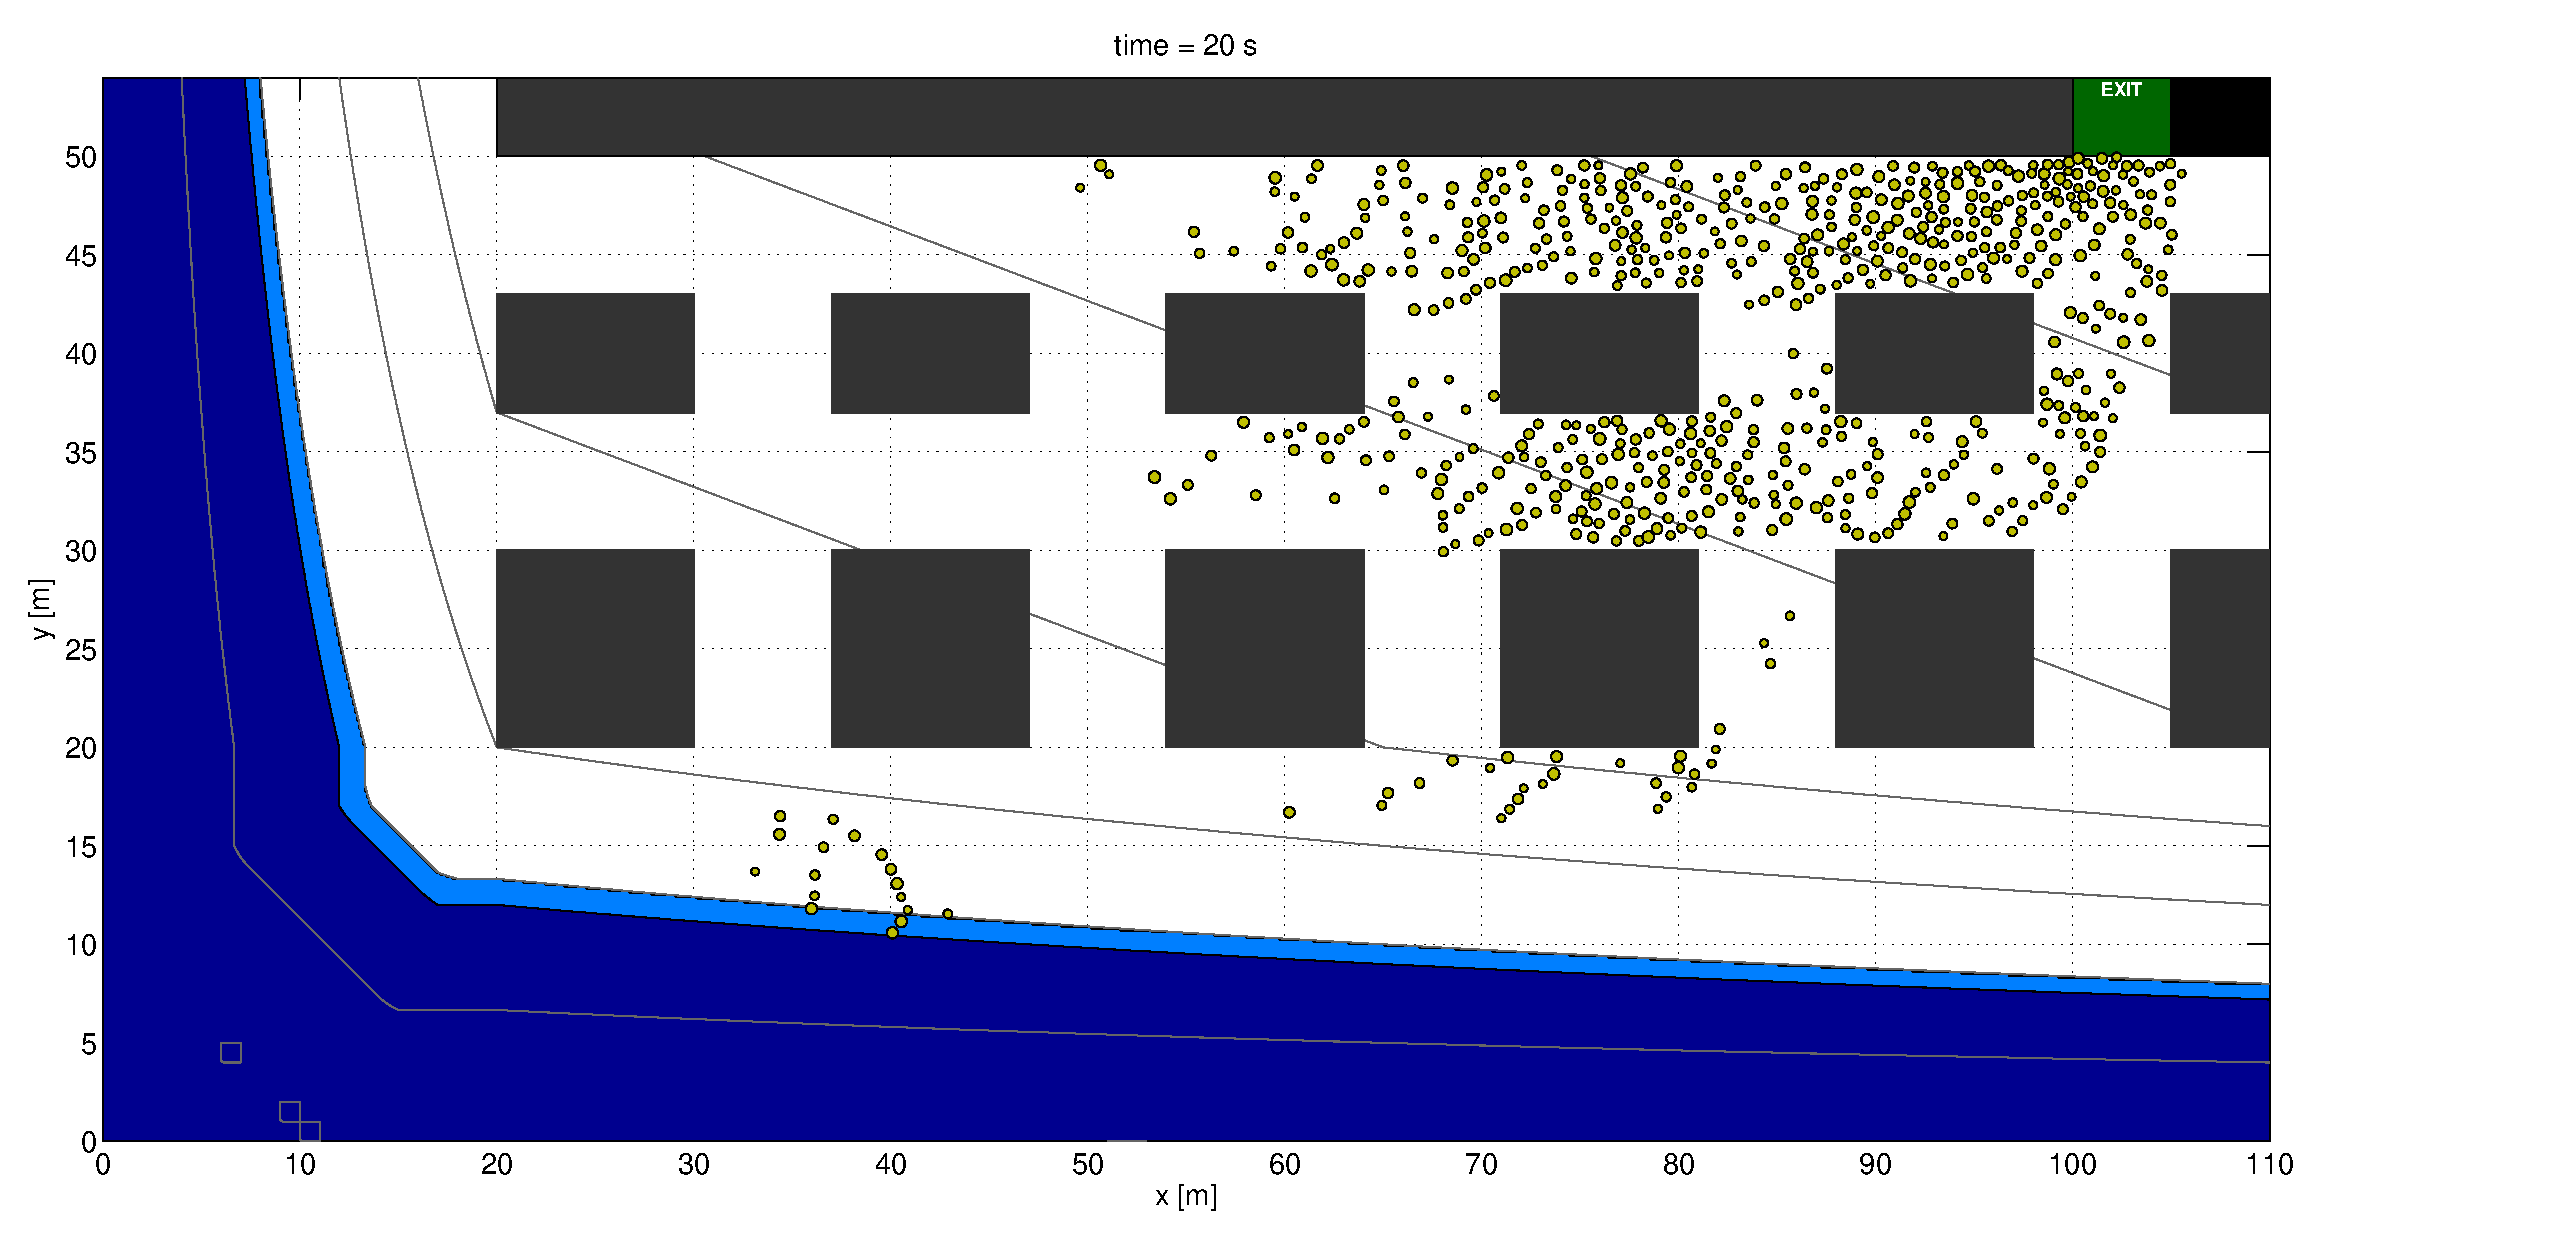
\includegraphics[width=1.1\textwidth]{figures/BeachEvacuationOneExitStreetWidth7_Flood0_1_002000.eps}
	\caption{Wide beach house setup: different time steps show the approach of the flood and the escaping pedestrians.}
	\label{fig:beach_1}
\end{figure}

\begin{figure}
	\centering
	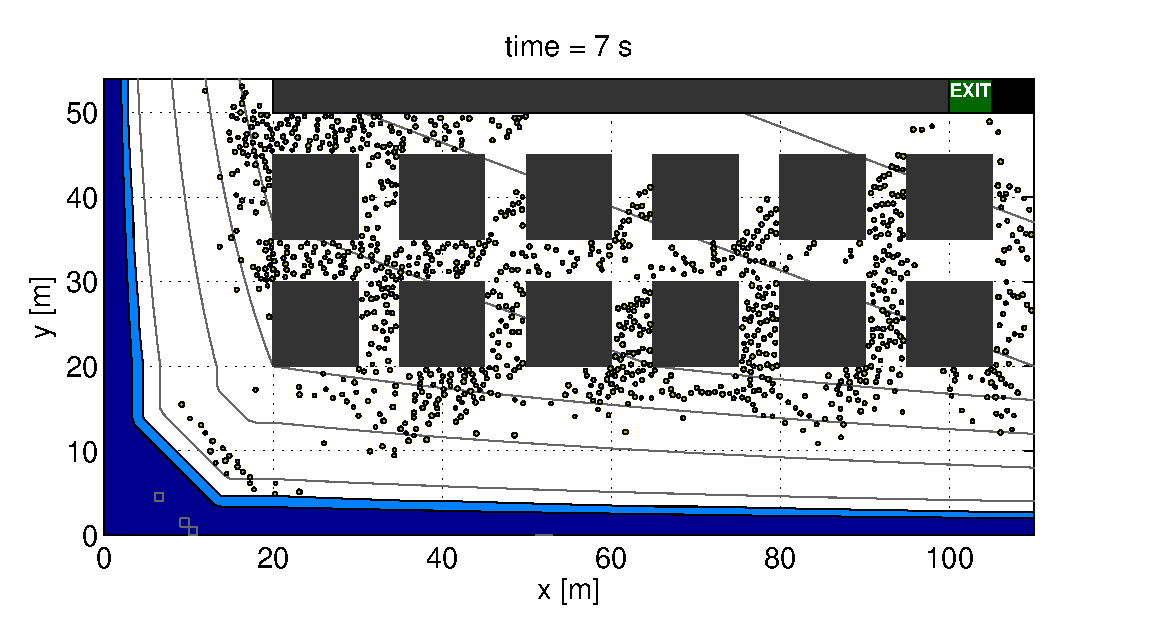
\includegraphics[width=1.1\textwidth]{figures/BeachEvacuationOneExitStreetWidth5_Flood0_1_000700.eps}
	\qquad
	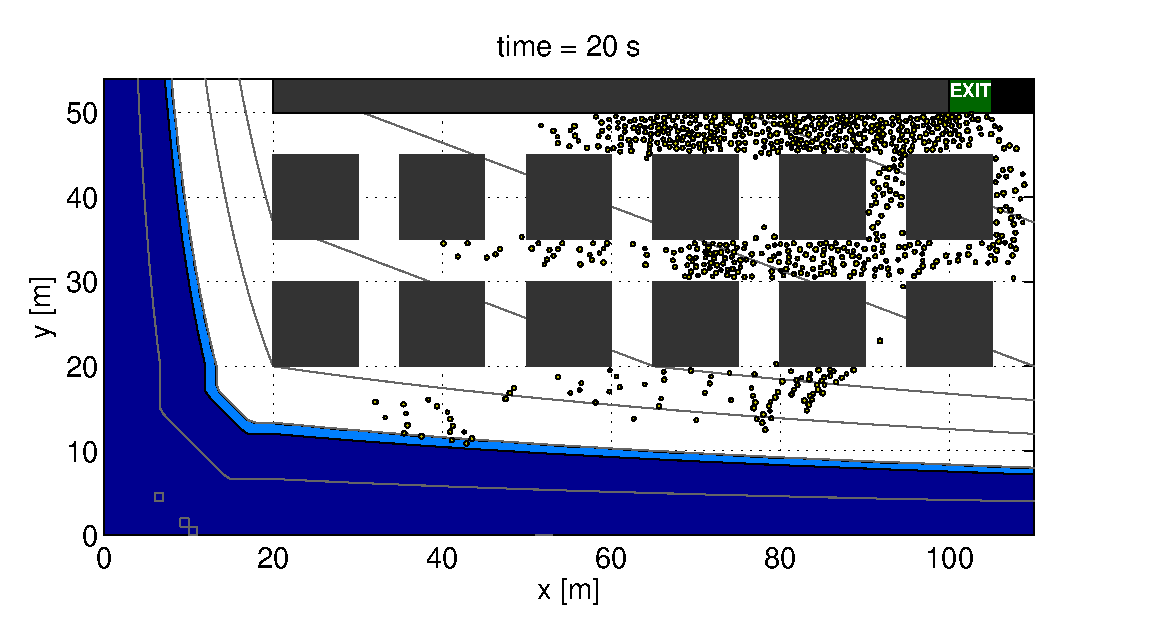
\includegraphics[width=1.1\textwidth]{figures/BeachEvacuationOneExitStreetWidth5_Flood0_1_002000.eps}
	\caption{Intermediate beach house setup: different time steps show the approach of the flood and the escaping pedestrians.}
	\label{fig:beach_2}
\end{figure}

\begin{figure}
	\centering
	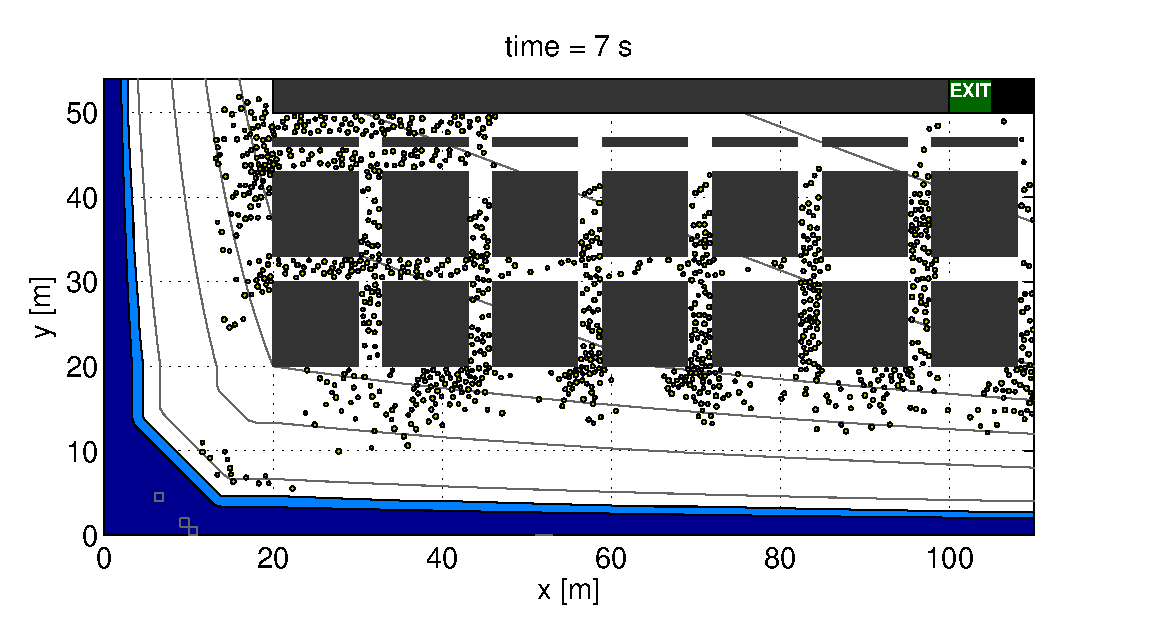
\includegraphics[width=1.1\textwidth]{figures/BeachEvacuationOneExitStreetWidth3_Flood0_1_000700.eps}
	\qquad
	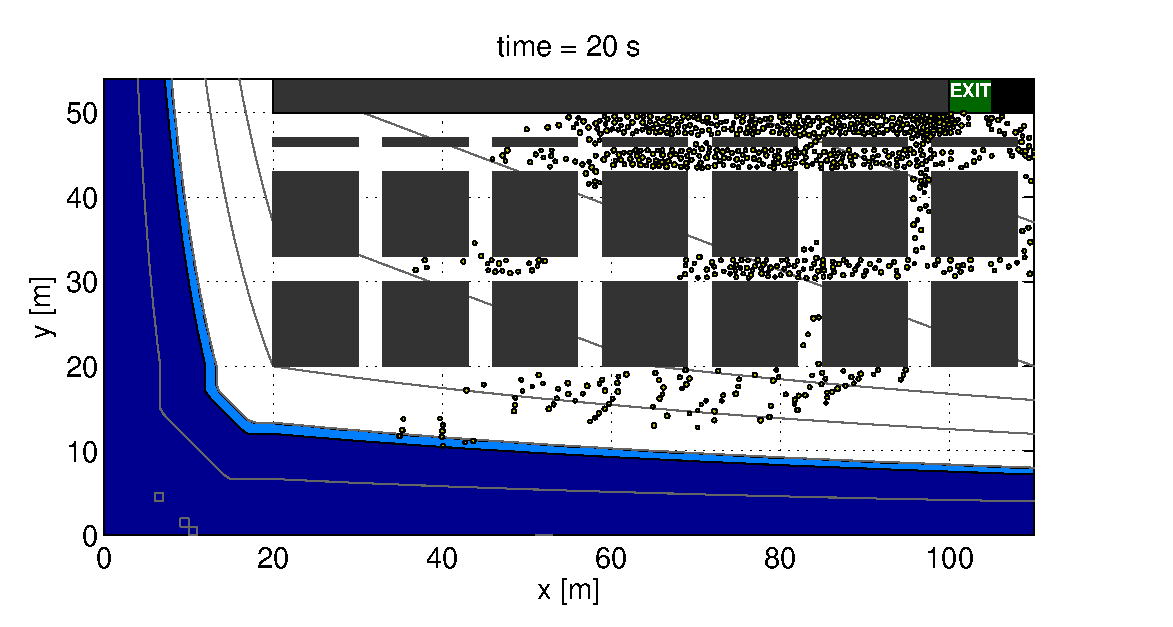
\includegraphics[width=1.1\textwidth]{figures/BeachEvacuationOneExitStreetWidth3_Flood0_1_002000.eps}
	\caption{Narrow beach house setup: different time steps show the approach of the flood and the escaping pedestrians.}
	\label{fig:beach_3}
\end{figure}

\begin{figure}
	\centering
	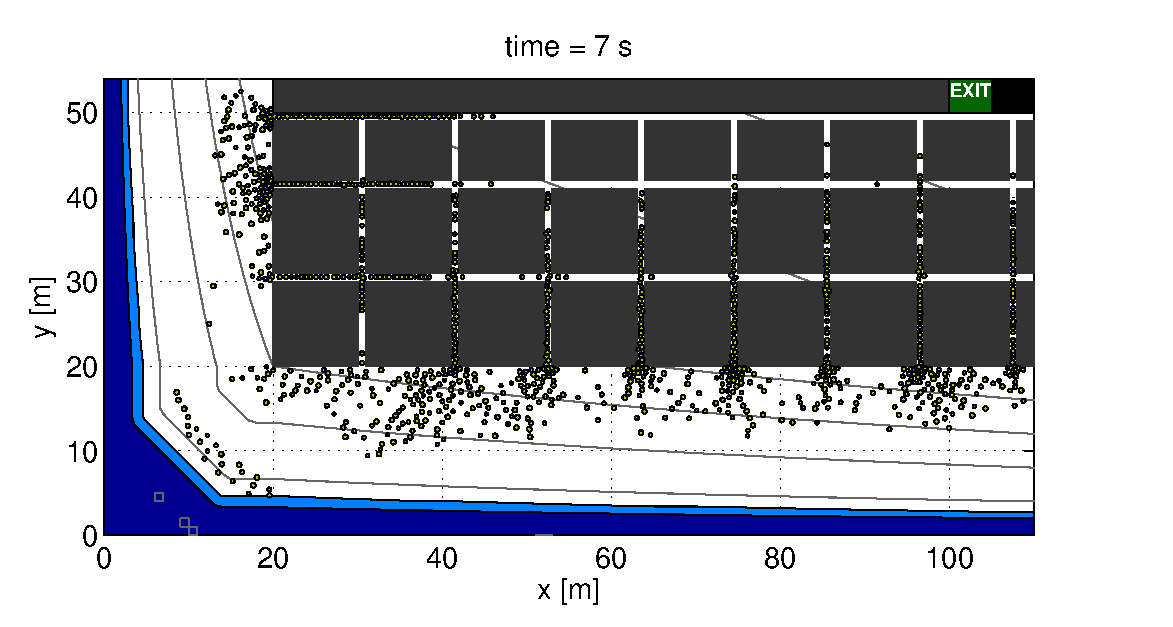
\includegraphics[width=1.1\textwidth]{figures/BeachEvacuationOneExitStreetWidth1_Flood0_1_000700.eps}
	\qquad
	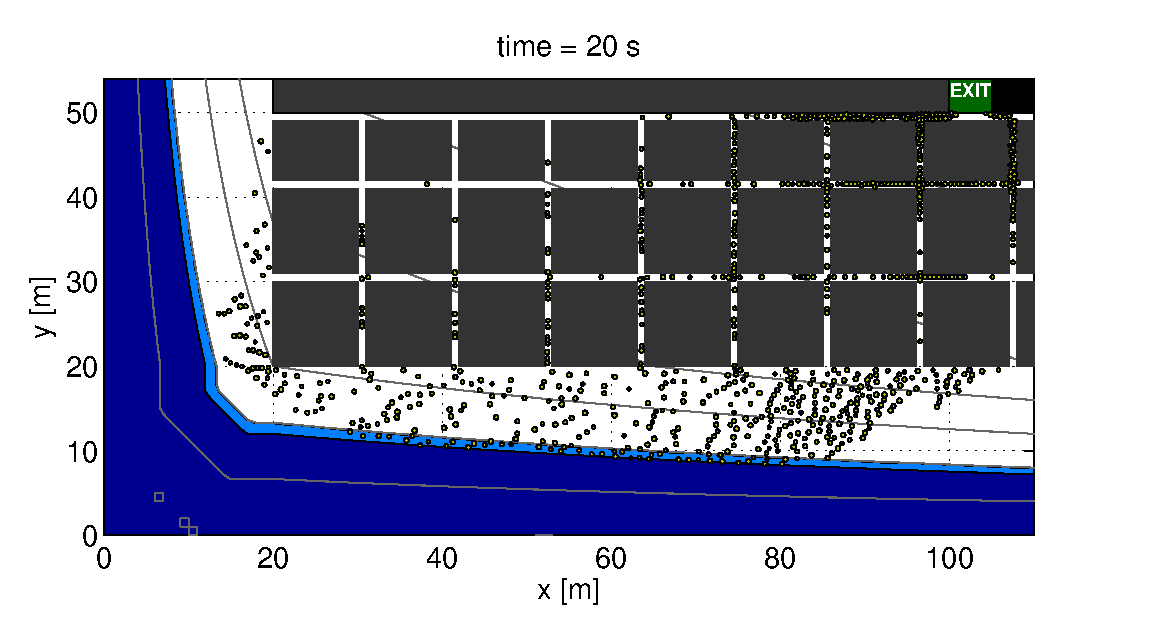
\includegraphics[width=1.1\textwidth]{figures/BeachEvacuationOneExitStreetWidth1_Flood0_1_002000.eps}
	\caption{Very narrow beach house setup: different time steps show the approach of the flood and the escaping pedestrians.}
	\label{fig:beach_4}
\end{figure}

\section{Summary and Outlook}


\section{References}


\bibliographystyle{plainnat}
%\bibliography{/Users/fabio/ETH/Vorlesungen/SOCIAL_MODELING/reportTemplate/bib/socialmodelling}


\begin{thebibliography}{3}
\providecommand{\natexlab}[1]{#1}
\providecommand{\url}[1]{\texttt{#1}}
\expandafter\ifx\csname urlstyle\endcsname\relax
  \providecommand{\doi}[1]{doi: #1}\else
  \providecommand{\doi}{doi: \begingroup \urlstyle{rm}\Url}\fi

\bibitem[Graf and Krebs(2010)]{Graf}
D.~Graf and M.~Krebs.
\newblock Train boarding platform simulation.
\newblock Modelling and Simulating Social Systems with MATLAB, ETHZ, 2010.

\bibitem[Helbing et~al.(2000)Helbing, Farkas, and Vicsek]{Helbing2000}
D.~Helbing, I.~Farkas, and T.~Vicsek.
\newblock Simulating dynamical features of escape panic.
\newblock \emph{Nature}, 407\penalty0 (6803):\penalty0 487--490, 2000.

\bibitem[Kneidl and Borrmann(2011)]{Kneidl}
A.~Kneidl and A.~Borrmann.
\newblock How do pedestrians find their way? results of an experimental study
  with students compared to simulation results.
\newblock In \emph{Conference on Emergency Evacuation}. Warsaw, Poland, 2011.

\end{thebibliography}



\end{document}  



 
